\chapter{Interferometric stabilisation of reservoir cavity}

\label{ch-stabilisation}

%%%%%%%%%% INTRODUCTION %%%%%%%%%%

\section{Introduction}

In this introductory section, the concept of interferometry is presented. As the name of the chapter suggests, this technique is used to stabilise the reservoir cavity. The reason why an optical cavity needs stabilisation will appear clearer later, but basically, this is due to the fact that light is a wave and that it can interfere with itself inside the cavity. Moreover, it will be shown that the interferometric properties are wavelength dependent. Since several wavelengths coexist inside the reservoir, this gives a first glimpse on the complexity entailing its stabilisation. To gain some insight on interferometry, and before moving on to the study of an actual ring cavity, the features of the well known \gls{fp} interferometer are recalled. After that, it is shown that the properties studied for the \gls{fp} can be translated to ring cavities with close to no modification. Finally, under the light of the basic notions of interferometry developed, the difficulties linked to the stabilisation of the reservoir cavity, which is at the heart of the scheme introduced in this thesis, are presented.

%%% FABRY-PEROT INTERFEROMETER %%%

\subsection{Fabry-Perot interferometer}

The \gls{fp} plays an important role in modern optics as it is really ubiquitous. This can be explained by the fact that, despite its great simplicity, it can reach good performance using high reflectivity mirrors, which can be produced using recent technologies. In practice, a \gls{fp} cavity is simply made of two mirrors facing each other as can be viewed in figure \ref{fp}. One can see the two mirrors, represented by the vertical black lines, and the different electric fields. The resonance condition, namely the situation where the transmitted electric field $E_{\text{t}}$ is maximum, can be seen intuitively as a situation where the intra-cavity field $E_1$ is in phase with the incident field $E_{\text{in}}$, which leads to the build up of an intra-cavity standing wave. On the other hand, the anti-resonance condition is met when $E_{\text{in}}$ and $E_1$ are out of phase. The transmissivity of the \gls{fp} interferometer, which is defined as the ratio $|E_{\text{t}}|^2/|E_{\text{in}}|^2$, is given by \cite{Perot1899}:

\begin{equation}
	\mathcal{T}(\omega) = \frac{1}{1+\mathcal{F}\sin^2{\left(\frac{\omega}{\text{FSR}}\right)}}
	\label{transmissivity}
\end{equation}

In this expression, $\mathcal{F}$ is the finesse of the cavity, $\omega$ is the angular frequency of the incident electric field, and FSR is the \acrlong{fsr} of the cavity. In a stationary regime, the energy inside the cavity does not evolve, therefore the energy carried by the incident electric field $E_{\text{in}}$ can either be transmitted or reflected, which implies that the reflectivity of the cavity which is defined as the ratio $|E_{\text{ref}}|^2/|E_{\text{in}}|^2$ is simply given by:

\begin{equation}
	\mathcal{R}(\omega) = 1 - \mathcal{T}(\omega)
	\label{reflectivity}
\end{equation}

\begin{figure}[h]
	\centering
	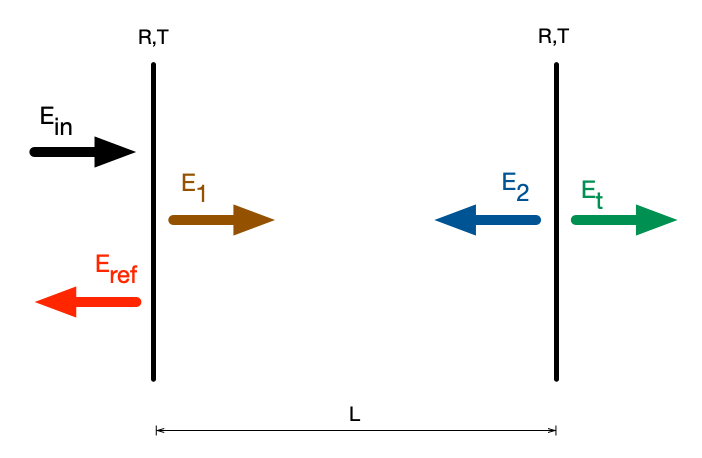
\includegraphics[width=.65\textwidth]{fp}
	\caption{Schematic representation of a \acrlong{fp} interferometer. $E_{\text{in}}$ is the incident electric field, $E_{\text{ref}}$ is the reflected electric field, $E_{\text{t}}$ is the transmitted electric field, $E_{1}$ is the intra-cavity electric field propagating from left to right, $E_{2}$ is the intra-cavity electric field propagating from right to left, $R$ and $T$ are the reflectivity and transmissivity of the two identical mirrors and $L$ is the distance between them.}
	\label{fp}
\end{figure}

In figure \ref{fp-tf}, the transmissivity (right) and reflectivity (left) of a lossless \gls{fp} can be viewed. These graphs exhibit peaks with a periodicity equal to the \gls{fsr} in the spectral domain. Recalling that $\text{FSR} = c/(2nL)$, one can see that the \gls{fsr} is linked to the length of the cavity, with $c$ the speed of light and $n$ the refractive index of the medium that could be present between the two mirrors ($nL$ is the optical path length). The finesse $\mathcal{F}$ is related to the width of the peaks and depends on the reflectivity of the mirrors as $\mathcal{F} = 4R/(1-R)^2$. As the reflectivity of the mirrors approaches 1, the finesse becomes large, and the peaks get narrow. On the other hand, with a lower reflectivity, more energy can leak out of the cavity even outside the resonance condition. Seeing the broadening of the peaks as energy leakage will be useful when drawing a parallel between \gls{fp} and ring cavity interferometers.

\begin{figure}[h]
	\centering
	\begin{subfigure}{.5\textwidth}
		\centering
		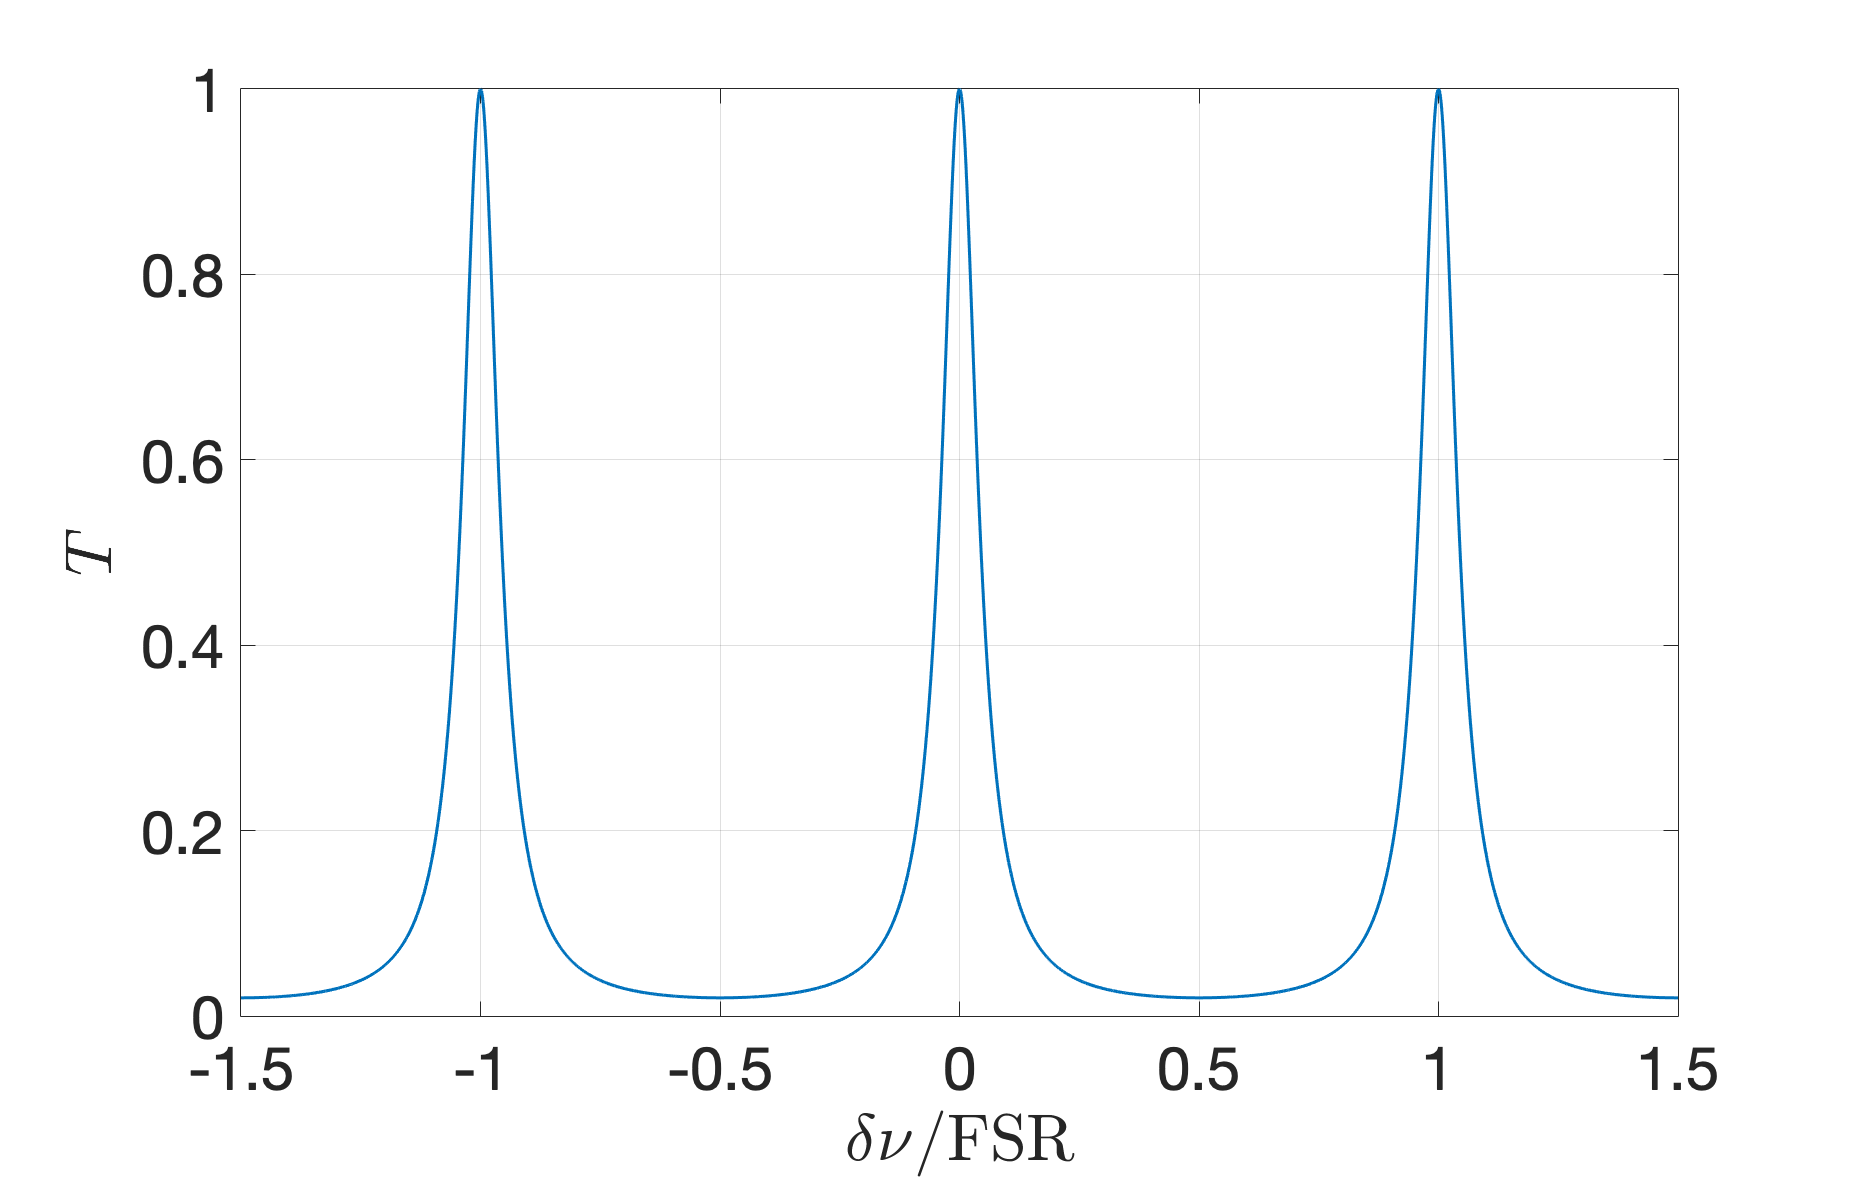
\includegraphics[width=\textwidth]{fp-trans-tf}
	\end{subfigure}%
	\begin{subfigure}{.5\textwidth}
		\centering
		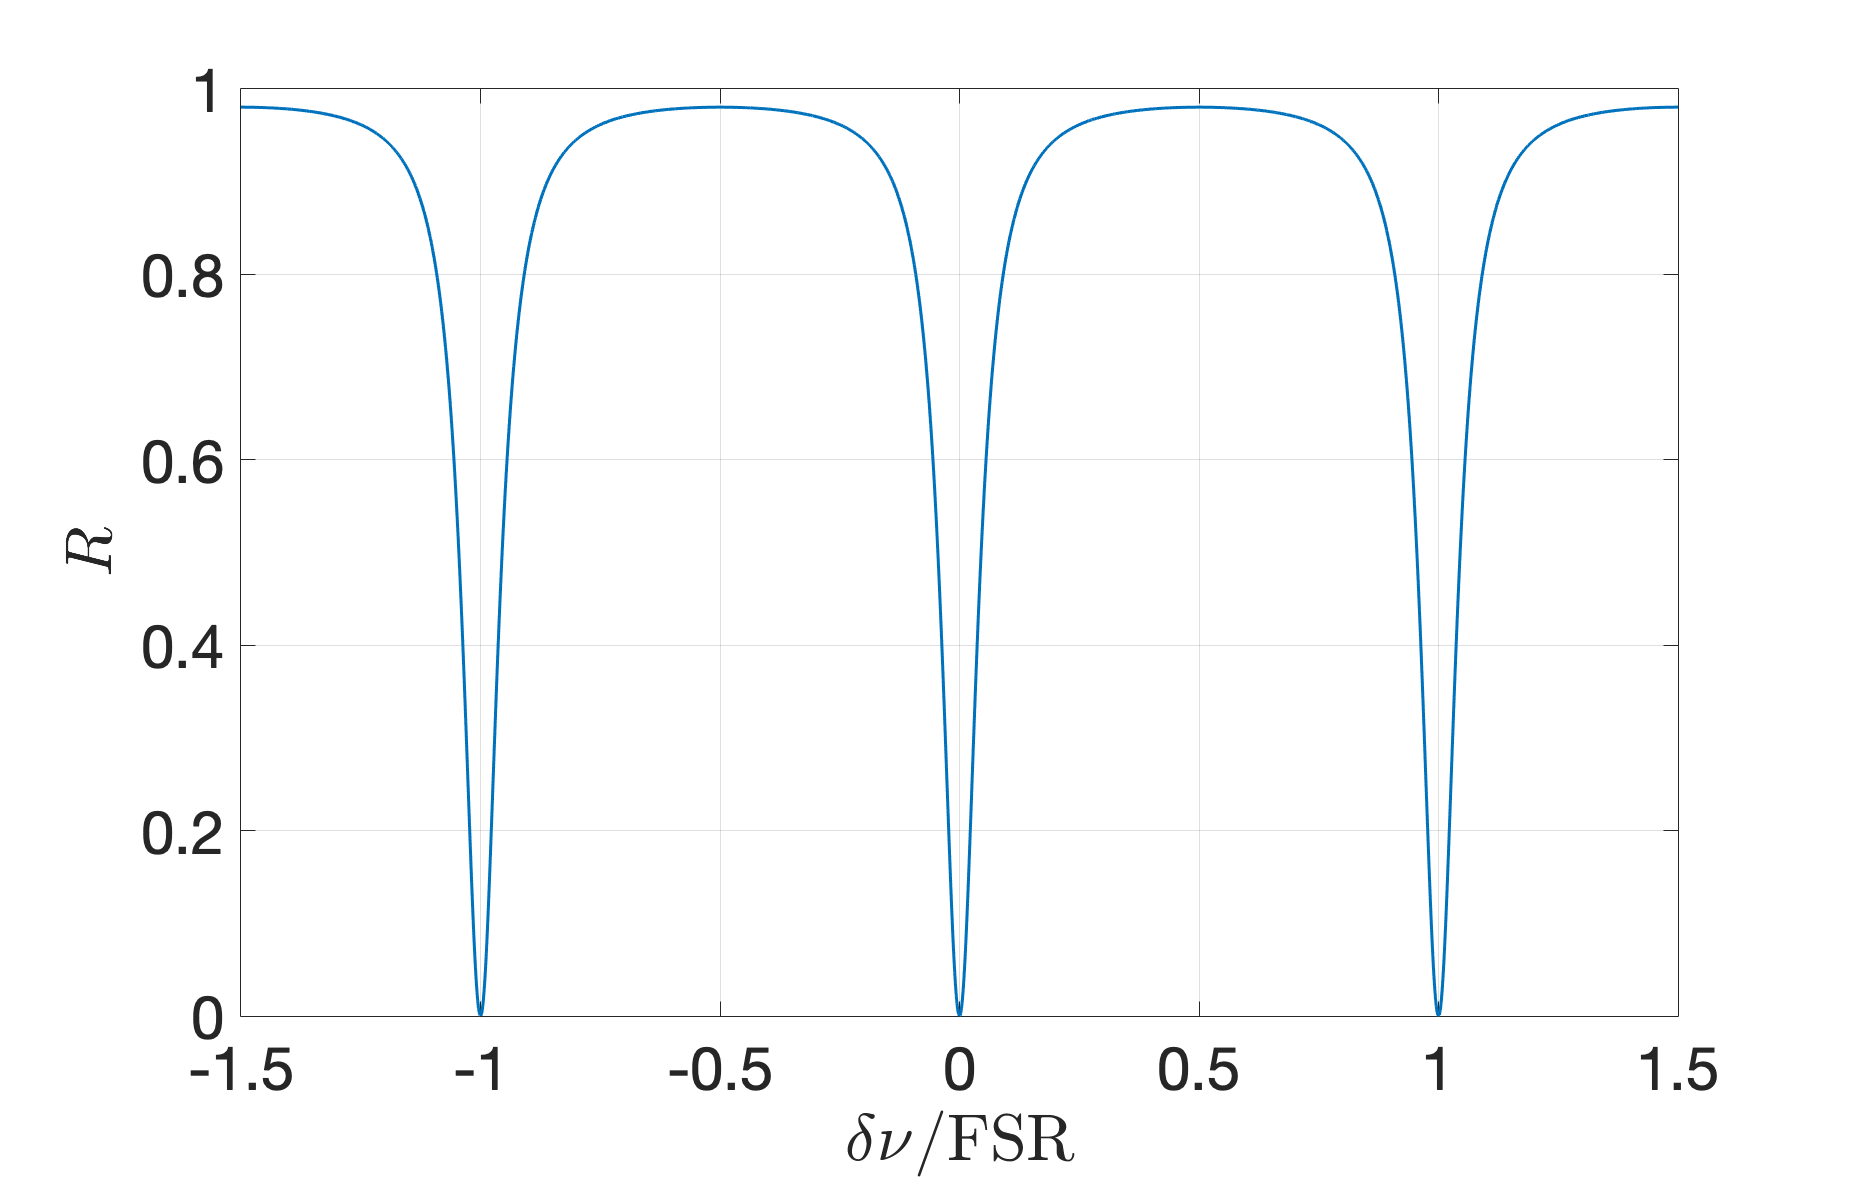
\includegraphics[width=\textwidth]{fp-ref-tf}
	\end{subfigure}
	\caption{Transmissivity $\mathcal{T}$ (left) and reflectivity $\mathcal{R}$ (right) of the cavity. Finesse $\mathcal{F}=50$. $\delta \nu$ denotes the deviation from a resonant frequency.}
	\label{fp-tf}
\end{figure}

Equation \eqref{transmissivity} and \eqref{reflectivity} indicate that $\mathcal{T}$ and $\mathcal{R}$ depend on $\omega/\text{FSR}$. This value can be rearranged as:

\begin{equation}
	\frac{\omega}{\text{FSR}} = kL = \phi
\end{equation}

Where $k$ is the wave number defined as $n \omega/c$ and $\phi$ is the phase acquired by the electric field when propagating along the cavity. Therefore, by measuring the transmitted or reflected power, one can gain information about the phase (modulo $\pi$, because the periodicity of $\mathcal{T}$ and $\mathcal{R}$ in the phase domain is $\pi$) of the electric field. This is the idea underlying interferometry.

%%% RING CAVITY %%%

\subsection{Ring cavity}

\label{subsec-ring-cavity}

A ring cavity exhibits the same behaviour as a \gls{fp} interferometer. The structure of a ring cavity interferometer is displayed in figure \ref{cavity_vs_fp}. This is a fibre-based setup in which the incident electric field $E_{\text{in}}$ penetrates the cavity from the left through a coupler. $E_{\text{ref}}$ denotes the electric field exiting the cavity and $E_1$ and $E_2$ refer to the fields entering and leaving the fibre loop, respectively. The nomenclature for the fields was chosen in such a way that the analogy with the \gls{fp} cavity can be understood. Indeed, one could see the coupler acting as the leftmost mirror from the figure \ref{fp}, and the fibre loop as the one on the right side because it turns $E_1$ into $E_2$ and dissipates energy through fibre losses, whereas for the mirror it was by leakage out of the lossless \gls{fp} cavity.

\begin{figure}[h]
	\centering
	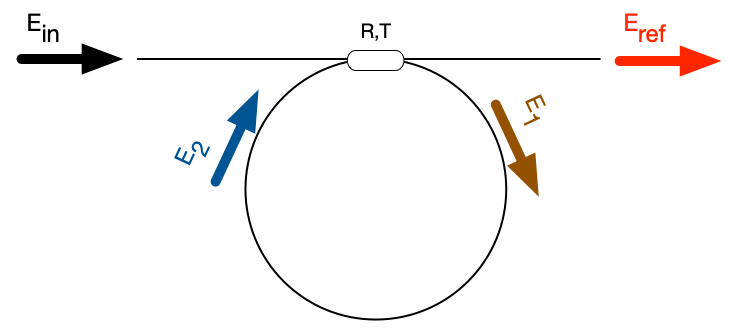
\includegraphics[width=.7\textwidth]{cavity_vs_fp}
	\caption{Schematic view of a ring cavity.}
	\label{cavity_vs_fp}
\end{figure}

Because of the similarities between ring cavities and \glspl{fp}, the former show the same transmissivity and reflectivity as the latter. Therefore, by measuring the reflected power, one can determine the phase acquired by the electric field inside the cavity.

%%% Interferometric properties of the reservoir cavity %%%

\subsection{Interferometric properties of the reservoir cavity}

The basic principle of interferometry has been introduced through the presentation of the \gls{fp} interferometer, and in the discussion that followed, it has been shown that a ring cavity, such as the reservoir cavity studied in this thesis, can be used as an interferometer. Moreover, it has also been shown that $\mathcal{R}$ depends on the frequency (or wavelength) and on the length of the cavity and that the phase acquired by the incident electric field after one round trip could be determined by studying the reflected power.\\

In the reservoir cavity, many different wavelengths coexist because they encode the different neurons. Furthermore, after each round trip, the respective phase acquired by each neuron should be a constant, as shown on equation \eqref{model-reservoir}. Recalling the phase matrix $\mathbf{\Phi}$ defined in equation \eqref{phase-matrix}, the phase factor multiplying the $k^{\text{th}}$ neuron is given by $\Phi_{kk} = \exp{(i\phi_k)}$.	The phase $\phi_k$ is given by:

\begin{equation}
	\phi_k = \beta(\omega+k\Omega) L
\end{equation}

With $\beta$ the fibre wave number, $\omega+k\Omega$ the angular frequency of the $k^{\text{th}}$ neuron and $L$ the length of the fibre loop. Because $k\Omega \ll \omega$, the wave number can be Taylor expanded: 

\begin{equation}
	\beta(\omega+k\Omega) = \beta(\omega) + \left. \frac{\partial\beta}{\partial\omega}\right\rvert_\omega k\Omega + \mathcal{O}\left((k\Omega)^2\right)
\end{equation}

By rewriting $\beta(\omega)$ and $\partial\beta/\partial\omega\rvert_\omega$ as $\beta_0$ and $\beta_1$, respectively, as it is often done in the literature, the acquired phase is given by:

\begin{equation}
	\phi_k \approx \beta_0 L + k \beta_1 \Omega L = \phi_0 + k \phi_1
\end{equation}

This means that if $\phi_1$ is an integer multiple of $\pi$, the phase factor multiplying all the neurons will be the same up to a sign:

\begin{equation}
	e^{i(\phi_0+k\phi_1)} = e^{i\phi_0}e^{ikm\pi} =(-1)^{km} e^{i\phi_0}, \quad m \in \mathbb{Z}
\end{equation}

A periodicity of $\pi$ and not $2\pi$ is considered here, because as claimed before, an interferometer can only inform about a phase modulo $\pi$. Looking for an acquired phase equal to $\pi$ is the approximately the same as taking a modulation frequency $\Omega$ for the \gls{pm} which is an integer multiple of the \gls{fsr}. Indeed, by considering $\beta_1 \approx n/c$, one can find:

\begin{equation}
	\beta_1 \Omega L \approx \frac{\Omega n L}{c} = m\pi \longrightarrow \Omega \approx \frac{m\pi c}{n L} = m2\pi ~\text{FSR}
\end{equation}

This is a legitimate assumption given the fact that in the region of interest the curve of $\beta(\omega)$ computed using the Sellmeier relations \cite{Bruckner,malitson1965interspecimen} exhibits negligible nonlinearity.\\

It is not critical to modulate the phase at an angular frequency $\Omega$ which is an integer multiple of the \gls{fsr}, the reservoir can in fact operate in different regimes. Those considerations were presented to better understand the physics underlying the phase management of the reservoir.\\

To be able to function as a \rcer, the reservoir has to be stabilised because during its operation, perturbations coming from various sources, such as mechanical constraints or temperature changes for example, can induce a phase fluctuation, which affects the \rcer performances. Classical cavity stabilisation strategies rely on interferometric properties to ensure the regulation. They use \gls{pid} regulators to maintain the reflected power at a reference level, which can be related to a phase, knowing the reflectivity of the cavity. A technical issue inherent to this scheme is the fact that the incident electric field used to stabilise the cavity is also modulated in intensity because it is carrying the input data processed by the \rcer, which has the consequence of deteriorating the reflected power signal based on which the cavity is stabilised. A possible solution is to use the \pdh stabilisation technique, which is an advanced cavity stabilisation technique leading to better performances. These two stabilisation techniques are presented in sections \ref{subsubsec-cavity-stab} and \ref{subsec-pdh-technique}, respectively.

%%%%%%%%%% EXPERIMENTAL SETUP %%%%%%%%%%

\section{Experimental setup}

In this section, the experimental setup employed to physically implement the \gls{wdm} \gls{prc} is presented. First, it is detailed based with the help of the schematic representation of figure \ref{exp-setup}. Then, technical data about the devices involved in the experiment are given.

\begin{figure}[h]
	\centering
	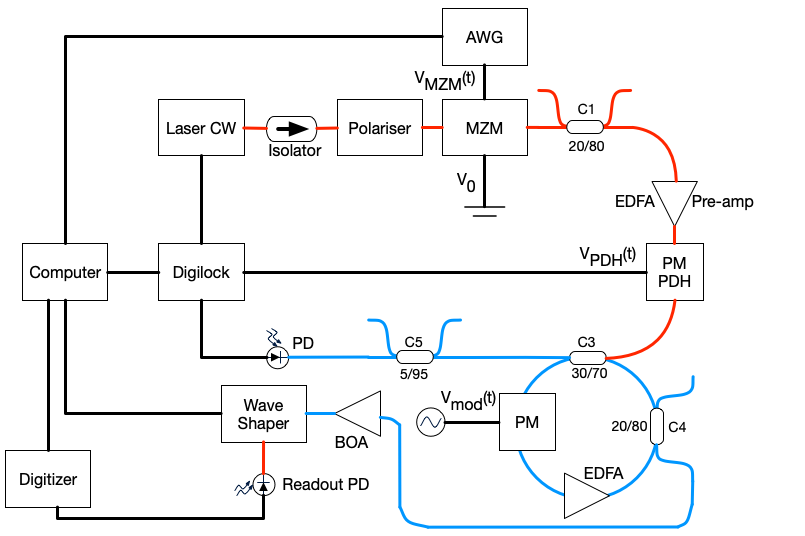
\includegraphics[width=\textwidth]{exp-setup}
	\caption{Schematic representation of the experimental setup. Red and blue lines: polarisation maintaining single mode fibres with only one or several wavelengths coexisting, respectively, black lines: electrical connections, CW: continuous wave, AWG: arbitrary wave generator, MZM: MAch-Zehnder Modulator, EDFA: Erbium Doped Fibre Amplifier, PM: phase modulator, PM - PDH, phase modulator involved in the \pdh technique, PD: photodiode, C$x$: coupler number $x$, BOA: Booster Optical Amplifier.}
	\label{exp-setup}
\end{figure}

The setup presented here is mostly an update on the one presented in \cite{AkroutAkram2016Pprc}. In figure \ref{exp-setup}, electrical wires and single mode polarisation maintaining fibres are represented using black and coloured lines, respectively.  The light source of the setup is a narrow band continuous laser, which sends a single wavelength $\lambda_0 =$ 1555 nm to the reservoir. The light goes through an isolator that prevents any backward reflection towards the laser source and then enters a polariser that ensures that only one linear polarisation mode is present inside the setup. This needs to be done to avoid any potential coupling between the two polarisation modes, and because the optoelectronic devices involved in the experiment, such as the \gls{mzm} and the \glspl{pm}, are polarisation dependent. The electric field then enters the \gls{mzm} which is driven by the time dependent voltage $V_{\text{MZM}}(t)$. This signal is generated by an \gls{awg} based on the input time series $u(n)$ sent by the computer running the experiment. Since the transfer function of the \gls{mzm} is nonlinear, the signal $V_{\text{MZM}}$ can be precompensated in order to counteract the nonlinearity. Without precompensation, the voltage $V_{\text{MZM}}(t)$ is simply given by $\beta \tilde{u}(t)$, with $\beta$ the input gain $\in [0,1]$ and $\tilde{u}(t)$ the \textit{sample and hold} version of $u(n)$ already introduced in the previous chapter. A bias tension $V_0$ can also be applied to the \gls{mzm} to change its average transparency. The transfer function of the \gls{mzm} is given by :

\begin{equation}
	\sin{ \left(\frac{\pi}{2} \left(\frac{V_{\text{MZM}}(t)}{V_{\pi,\text{RF}}} + \frac{V_0}{V_{\pi, \text{DC}}} \right) \right)}
\end{equation}

With $V_{\text{MZM}} \in [-\beta V_{\pi,\text{RF}},\beta V_{\pi,\text{RF}}]$, and $V_{\pi,\text{RF}}$ and $V_{\pi,\text{DC}}$ the dynamic and static characteristic voltages of the \gls{mzm}, respectively. The modulated electric field is then pre-amplified using an \gls{edfa}, and undergoes a first phase modulation. This is required to be able to implement the \gls{pdh} stabilisation technique. The \gls{pm} is driven by the alternative voltage $V_{\text{PDH}} = A_{\text{PDH}} \sin{(\Omega_{\text{PDH}}t)}$ supplied by the \textit{Toptica Digilock 110} feedback controller denoted "Digilock" on the figure. This device handles every aspect related to the stabilisation of the reservoir, which is why it needs to be connected to the photodiode "PD" and to the laser, which are both involved in the regulation of the cavity, as it is explained in section \ref{subsubsec-cavity-stab}. The electric field then enters the reservoir through the coupler "C3". The reservoir cavity is made of the fibres of the different couplers and is around \SI{18}{m} long. At this point, the colour used to represent the optical fibres changes from red to blue to indicate that inside the reservoir, several wavelengths are present whereas before the coupler there was only one. Inside the reservoir, the \gls{pm} is used to mix the different frequencies and is driven by an external alternative voltage $V_{\text{mod}}(t) = A_{\text{mod}} \sin{ (\Omega_{\text{mod}} t)}$. To allow a clear distinction between the different sidebands without degrading the achievable modulation depth, the modulation frequency $\pulsefreq{\Omega_{\text{mod}}}$ is around 20 GHz. This allows the existence of 13 neurons inside the cavity (6 sidebands on both sides of the central frequency) with wavelengths going from \SIrange{1.554}{1.556}{\micro\metre} in the telecom C-band. The \gls{pm} introduces insertion losses that are compensated using the \gls{edfa}, whose pump current is adjusted to tune the feedback gain $\alpha$ that appears in equation \eqref{model-reservoir}. The electric field exiting the reservoir at the level of the coupler "C3" towards the photodiode "PD" is the reflected field, according to what was discussed in section \ref{subsec-ring-cavity}. The electric field finally illuminates the photodiode "PD", and produces a voltage proportional to its intensity, called the reflected power. This measured signal enters the Digilock where it is used electronically post-preocessed in order to recover the \pdh signal, whose properties are presented in section \ref{subsec-pdh-technique}. Based on the value of this signal, the Digilock outputs a control voltage that is applied to a piezoelectric crystal inside the laser cavity and that modifies its emission wavelength. The output of the reservoir exits the cavity thought the coupler "C4" and is amplified by a \gls{soa} called "BOA" for Booster Optical Amplifier to improve the \gls{snr}. A demultiplexing scheme allowing to obtain the value of each individual neuron at the same time has not been implemented yet. To overcome this limitation, the adjustable band-pass filter denoted "Wave Shaper" is used to record the evolution of only one neuron at a time. This implies that if one wants to compute the output of the reservoir $y(n)$, one has to run the same experiment once for each of the neuron, to program the Wave Shaper to filter out all the other sidebands and to save its evolution on the computer. Once this has been done, $y(n)$ can be reconstructed. As far as the learning procedure is concerned, it follows the same procedure as the one previously described, but modified to take this sequential measurements of the neurons into account. In terms of the devices used to perform this task, the photodiode "Readout PD" measures the intensity of each of the filtered neuron, and the "Digitizer" handles the conversion between continuous time dependent signals into time series usable by the computer. To conclude this description of the experimental setup, one should note that the couplers "C1" and "C5" are used in practice to monitor the electric fields when modifications are made to the optical table, and that the AWG, Digilock, Wave Shaper and Digitizer are all controlled by the computer. The technical specifications of the devices used in the experiment can be found in appendix \ref{app-data}.

%%%%%%%%%% CHARACTERISATION OF THE RESERVOIR %%%%%%%%%%

\section{Characterisation of the reservoir}

To be able to develop a reliable stabilisation scheme for the reservoir, some of its characteristics need to be studied as a preliminary work. First, one can gain important insights by modelling the transfer function of the reservoir. In this context, the transfer function is simply the reflectivity of the cavity as a function of the frequency of the incident wave. However, given the fact that the reservoir is a more complex ring cavity than the one depicted in section \ref{subsec-ring-cavity}, it will not exhibit the same behaviour as the one of a \gls{fp} cavity as displayed in figure \ref{fp-tf}. A mathematical model is first derived and the results it provides are compared to experimental transfer functions. After that, the experimental study of the effective losses is tackled. The effective losses are used in the model to take into account the fibre losses, the insertion losses of the \gls{pm} and the gain of \gls{edfa} using only one factor. Finally, an empirical relation between the modulation amplitude driving the intra-cavity \gls{pm} and its modulation depth is determined experimentally.

%%% TRANSFER FUNCTION OF THE CAVITY %%%

\subsection{Transfer function of the cavity}

As already claimed, in the context of cavity stabilisation, the transfer function is the reflectivity. When operating the reservoir, the reflected power which is proportional to the intensity of the electric field reflected by the cavity gives an indication on the phase of the field inside it, which implies that the regulation procedure relies on the measurement of this signal. \\

In figure \ref{schematic_reservoir}, the reservoir is represented with the different electric fields that turn out to be useful when studying the transfer function. The colour code for the fibres is the same as the one used previously. The incident electric field $\efield{in}$ enters the cavity through a coupler from the top left optical fibre. Inside the cavity, it is amplified by the \gls{edfa} and then is phase modulated. After that, a portion of the electric field exits the cavity through the coupler C4 to be read out. The light inside the cavity finally terminates its round trip.

\begin{figure}[h]
	\centering
	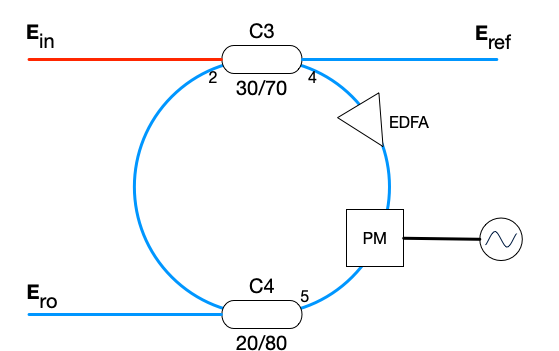
\includegraphics[width=.7\textwidth]{reservoir}
	\caption{Schematic representation of the reservoir.}
	\label{schematic_reservoir}
\end{figure}

% MATHEMATICAL MODEL %

\subsubsection{Mathematical model}

\label{subsubsec-tf-cavity}

In this section, a mathematical model for the transfer function is derived. To do so, the formalism introduced in section \ref{subsec-reservoir-model} needs to be used. This can be done because the basis vectors were chosen such that a neuron state vector $\mathbf{x}$ is formally equal to an electric field. Therefore, one should pay attention to the fact that when referring the a vectorial electric field $\mathbf{E}$, it denotes an electric field expressed in the abstract basis $\{ \hat{\mathbf{e}}_j | \hat{\mathbf{e}}_j = \exp{ (i (\omega+j\Omega_{\text{mod}}t)}, ~j\in [-\eta, \eta ] \}$ instead of the usual physical space $\{\mathbf{1}_x, \mathbf{1}_y,\mathbf{1}_z \}$. It is recalled that $\eta = \lfloor N/2 \rfloor$ is the variable introduced to iterate through through the neurons in more convenient way.\\

The transfer function $\mathbf{R}$ is defined as the link between the incident and reflected electric fields:

\begin{equation}
	\efield{ref} = \mathbf{R} ~\efield{in}
\end{equation}

Given the vectorial nature of $\efield{ref}$ and $\efield{in}$, the transfer function is in fact a transfer matrix in this particular context. Recalling that the laser only emits light at the center wavelength, the incident field $\efield{in}$ is given by:

\begin{equation}
	\efield{in} = E_0 \hat{\mathbf{e}}_0
\end{equation}

With $E_0$ being an arbitrary complex amplitude. Given the properties of the coupler C3, one finds:

\begin{equation}
	\begin{bmatrix}
		\efield{ref}\\
		\efield{4}
	\end{bmatrix} = \begin{bmatrix}
		\epsilon_1 & i\sqrt{1-\epsilon_1^2} \\
		i\sqrt{1-\epsilon_1^2} & \epsilon_1
	\end{bmatrix}
	\begin{bmatrix}
		\efield{in}\\
		\efield{2}
	\end{bmatrix} 
\end{equation}

Which yields to the following expression for the reflected field:

\begin{equation}
	\efield{ref} = \epsilon_1 \efield{in} + i \sqrt{1-\epsilon_1^2} \efield{2}
	\label{eq-ref}
\end{equation}

Let us now express $\efield{2}$ as a function of $\efield{in}$ to close the system. Using the transfer matrix of the coupler C4, $\efield{2}$ reads :

\begin{equation}
	\begin{bmatrix}
		\efield{2}\\
		\efield{ro}
	\end{bmatrix} = e^{-\gamma L} \begin{bmatrix}
		\epsilon_2\\
		\sqrt{1-\epsilon_2^2}
	\end{bmatrix} \efield{5} \Longrightarrow \efield{2} = \epsilon_2 e^{-\gamma L} \efield{5}
\end{equation}

With $\gamma$ the effective losses coefficient and $L$, the length of the reservoir. Since the system is in a linear regime, the position of the coupler C4 in the cavity has no influence on the losses and on the phase. This property manifests itself because mathematically, the transfer matrix of the coupler C4 and and the phase matrix $\mathbf{\Phi}$ commute. By defining $\xi \in [0,1]$ as the variable indicating the relative position of the \gls{pm} inside the cavity ($\xi = 0$ if it is at the beginning of the cavity, $\xi=1$ if it is at the end). The phase acquired  by the electric field inside the reservoir is now dependent on the position of the \gls{pm}. This leads to the definition of two new matrices $\mathbf{\Phi}_\xi$ and $\mathbf{\Phi}_{1-\xi}$, which are based on the phase matrix $\mathbf{\Phi}$. They are diagonal matrices, expressed as:

\begin{align}
	\Phi_{\xi,nn} &= \exp{ \left(i \beta (\omega+n\Omega_{\text{mod}}) \xi L \right)} \nonumber \\
	\Phi_{1-\xi,nn} &= \exp{ \left(i \beta (\omega+n\Omega_{\text{mod}}) (1-\xi) L \right)}
\end{align}

With $\beta (\omega+n\Omega_{\text{mod}})$ the dispersion relation of the fibre evaluated at the frequency of the $n^{\text{th}}$ neuron. Recalling the coupling matrix of the \gls{pm} $\mathbf{J}$, one can rewrite $\efield{5}$ as a function of $\efield{4}$:

\begin{equation}
	\efield{5} = \mathbf{\Phi}_{1-\xi} \mathbf{J} \mathbf{\Phi}_\xi \efield{4}
\end{equation}

Using the transfer matrix of the coupler C3, one can express $\efield{4}$ as a function of $\efield{in}$ and $\efield{2}$:

\begin{equation}
	\efield{4} = i\sqrt{1-\epsilon_1^2} \efield{in} + \epsilon_1 \efield{2}
\end{equation}

This yields to a closed equation to determine $\efield{2}$:

\begin{align}
	\efield{2} &= i\sqrt{1-\epsilon_1^2} \epsilon_2 e^{-\gamma L} \mathbf{\Phi}_{1-\xi} \mathbf{J} \mathbf{\Phi}_\xi \efield{in} + \epsilon_1 \epsilon_2 e^{-\gamma L} \mathbf{\Phi}_{1-\xi} \mathbf{J} \mathbf{\Phi}_\xi \efield{2} \nonumber \\
	\hookrightarrow \efield{2} &= i \sqrt{1-\epsilon_1^2} \epsilon_2 e^{-\gamma L} \left( \mathbf{I} - \epsilon_1 \epsilon_2 e^{- \gamma L} \mathbf{\Phi}_{1-\xi} \mathbf{J} \mathbf{\Phi}_\xi \right)^{-1} \mathbf{\Phi}_{1-\xi} \mathbf{J} \mathbf{\Phi}_\xi \efield{in}
\end{align}

Now that $\efield{2}$ has been determined, it is easy to compute $\efield{ref}$ using equation \eqref{eq-ref}:

\begin{align}
	\efield{ref} &= \epsilon_1 \efield{in} - (1-\epsilon_1^2) \epsilon_2 e^{-\gamma L} \left( \mathbf{I} - \epsilon_1 \epsilon_2 e^{- \gamma L} \mathbf{\Phi}_{1-\xi} \mathbf{J} \mathbf{\Phi}_\xi \right)^{-1} \mathbf{\Phi}_{1-\xi} \mathbf{J} \mathbf{\Phi}_\xi \efield{in} \nonumber \\
	\hookrightarrow \efield{ref} &= (\epsilon_1 \mathbf{I} - (1-\epsilon_1^2) \epsilon_2 e^{-\gamma L} \left( \mathbf{I} - \epsilon_1 \epsilon_2 e^{- \gamma L} \mathbf{\Phi}_{1-\xi} \mathbf{J} \mathbf{\Phi}_\xi \right)^{-1} \mathbf{\Phi}_{1-\xi} \mathbf{J} \mathbf{\Phi}_\xi) \efield{in}
\end{align}

This last equality reveals the expression of the transfer matrix $\mathbf{R}$:

\begin{equation}
	\boxed{\mathbf{R} = \epsilon_1 \mathbf{I} - (1-\epsilon_1^2) \epsilon_2 e^{-\gamma L} \left( \mathbf{I} - \epsilon_1 \epsilon_2 e^{- \gamma L} \mathbf{\Phi}_{1-\xi} \mathbf{J} \mathbf{\Phi}_\xi \right)^{-1} \mathbf{\Phi}_{1-\xi} \mathbf{J} \mathbf{\Phi}_\xi}
	\label{eq-tf-matrix}
\end{equation}

Even if this result is interesting, it cannot be measured directly since it involves electric fields instead of intensities. What is measured using a \gls{pd} is the reflectivity $\mathcal{R}$ linking the incident intensity to the reflected intensity. Recalling that the incident electric field is given by $\efield{in} = E_0 \hat{\mathbf{e}}_0$, the reflected electric field is given by:

\begin{equation}
	\efield{ref} = \mathbf{R}~\efield{in} = E_0\sum_{n=-\eta}^\eta R_{n,0} \hat{\mathbf{e}}_n
	\label{eq-reflected-vector}
\end{equation}

The sum in this formula is expressed using the numbering introduced in section \ref{subsec-reservoir-model} which is more natural for this kind of situation. As a reminder, instead of going through the indices from 1 to $N$, this alternative notation goes from $-\eta$ to $\eta$, with index 0 referring to the central neuron. Thus, the above equation basically means that $\efield{ref}$ is equal to $E_0$ multiplying the central column of $\mathbf{R}$.\\

The reflected intensity is given by:

\begin{equation}
	|\efield{ref}|^2 = |E_0|^2 \left(\sum_{n=-\eta}^\eta R_{n,0} \hat{\mathbf{e}}_n \right) \left(\sum_{m=-\eta}^\eta R_{m,0}^* \hat{\mathbf{e}}_m^* \right)
\end{equation}

This expression seems complicated at first sight, but it can be simplified by putting forward an experimental argument. First, let us consider the product $\hat{\mathbf{e}}_n \cdot \hat{\mathbf{e}}_m^*$, which is equal to $\exp{(i(n-m)\Omega_{\text{mod}}t)}$. If $m=n$, then the product is equal to one and the term $|R_n,0|^2$ has to be taken into account in the sum. On the other hand, if $m\neq m$, then product corresponds to a beating of the intensity at frequency $(n-m)\pulsefreq{\Omega_{\text{mod}}}$, which is an integer number of times approximately 20 GHz. However, as can be seen in the appendix \ref{app-data}, the bandwidth of the \gls{pd} is limited to 120 MHz. Therefore the \gls{pd} is not able to resolve the beating waves, which implies that when $m=n$, the signals do not contribute to the sum. This yields to a simplified version of the reflected intensity:

\begin{equation}
	|\efield{ref}|^2 = |E_0|^2 \sum_{n=-\eta}^\eta |R_{n,0}|^2
\end{equation}

The reflectivity of the reservoir is finally given by:

\begin{equation}
	\mathcal{R} = \sum_{n=-\eta}^\eta |R_{n,0}|^2
\end{equation}

Note that this model is solely valid when considering the evolution of the reservoir at time scales much larger than $2\pi / \text{FSR}$. This assumption ensures that one is working in a stationary regime with respect to the characteristic time-scale of the reservoir.

% EXPERIMENTAL RESULTS %

\subsubsection{Experimental results}

The adequacy of the analytical model just derived is assessed by comparing its predictions to experimental data. To capture data concerning transfer functions, one performs a \textit{sweep} using the Digilock. As already explained, the Digilock is connected to a piezoelectric crystal controlling the emission wavelength of the laser, whose shift is proportional to the applied tension. As a reminder, the transfer function is the reflectivity $\mathcal{R}$ as a function of $\omega$, therefore one needs to be able to scan the frequency domain. The sweep procedure allows to do it by applying a triangular periodic voltage to the piezoelectric, which leads to a proportional evolution of the emission wavelength of the laser. The frequency and amplitude of this signal are controlled by the Digilock interface. This procedure allows to plot the reflected power as a function of the time to observe its shape.\\

To relate the theoretical curves to raw data, one should express the link between the time and the angular frequency. Using a first order Taylor approximation, the angular frequency variation reads:

\begin{equation}
	\delta \omega = -\frac{2\pi c}{\lambda_0^2} \delta \lambda
\end{equation}

With $\lambda_0$ the central wavelength (1555 nm). In appendix \ref{app-data}, one can find that the piezoelectric tuning characteristic is equal 0.1 pm/V at a sweeping frequency of \SI{100}{\Hz}. Let us denote this value by $p$ and let us call $q$ the slope of the triangular voltage as a function of the time, which depends on the settings of the sweep. Multiplying those two constants provides a proportionality indicating the range of wavelengths spanned per unit of time. This yields to a link between time and angular frequency:

\begin{equation}
	\omega = - p q \frac{2 \pi c}{\lambda_0^2} t
	\label{eq-omega-vs-t}
\end{equation}

Below, comparisons between simulations and experimental data are shown for three different regimes. Since the theoretical reflectivity $\mathcal{R}$ is a ratio, it is comprised between 0 and 1. Therefore, it had to be rescaled in order to be compared with the reflected powers measured by the \gls{pd}.

\paragraph{First sideband at resonance} If the central neuron is at resonance, this means that $\omegamod$ is chosen such that the first sideband is at resonance as well. In other words, $\pulsefreq{\omegamod}$ is an integer number of times the \gls{fsr} of the cavity. This is displayed in figure \ref{tf_0}.

\begin{figure}
	\centering
	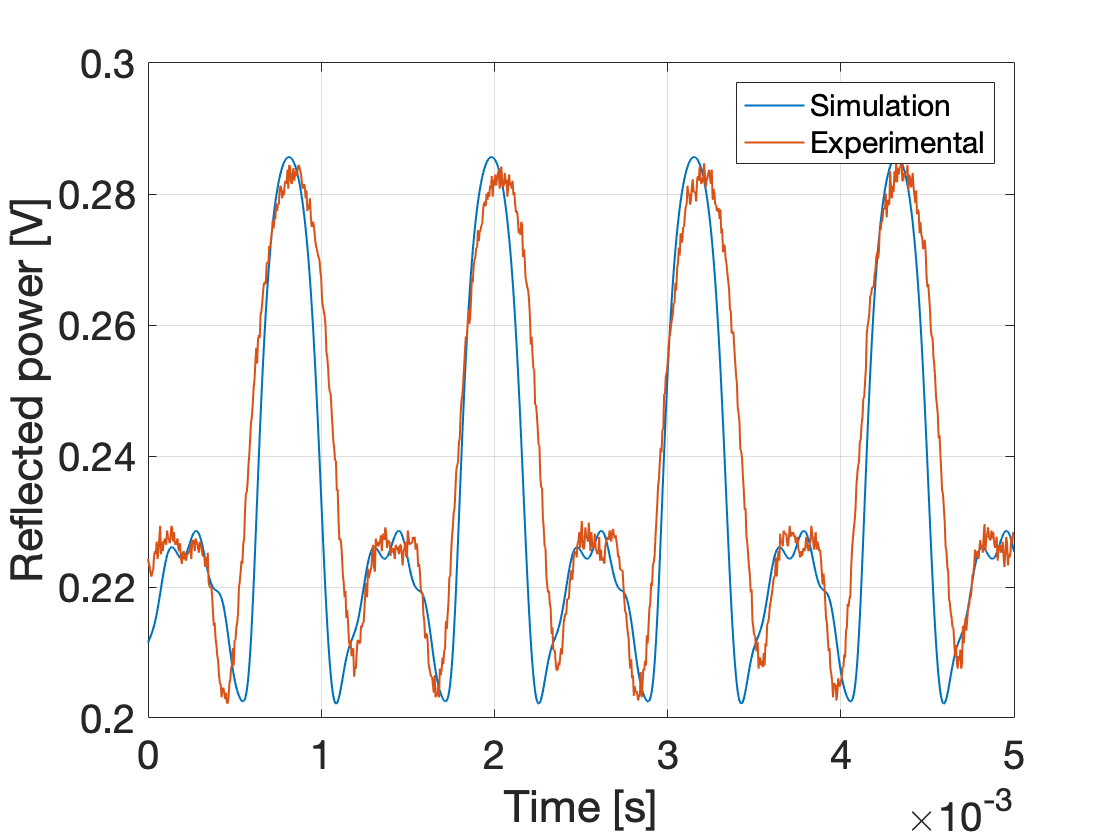
\includegraphics[width=.7\textwidth]{exp-tf-reservoir/tf_0.png}
	\caption{Reflected power [V] as a function of the time [s] during a sweep of the the piezo voltage. First sideband at resonance. $\Omega_{\text{mod}}$ = 19.99 GHz, modulation depth $m$ = 2, $\gamma = 0.0126~\text{m}^{-1}$. The theoretical curve has been rescaled in order to be compared with the experimental curve.}
	\label{tf_0}
\end{figure}

\paragraph{First sideband halfway between resonance and anti-resonance} $\omegamod$ is tuned such that $\pulsefreq{\omegamod}$ is an odd number of times the quarter of the \gls{fsr}. The experimental results are given on the figure \ref{tf_25}.

\begin{figure}
	\centering
	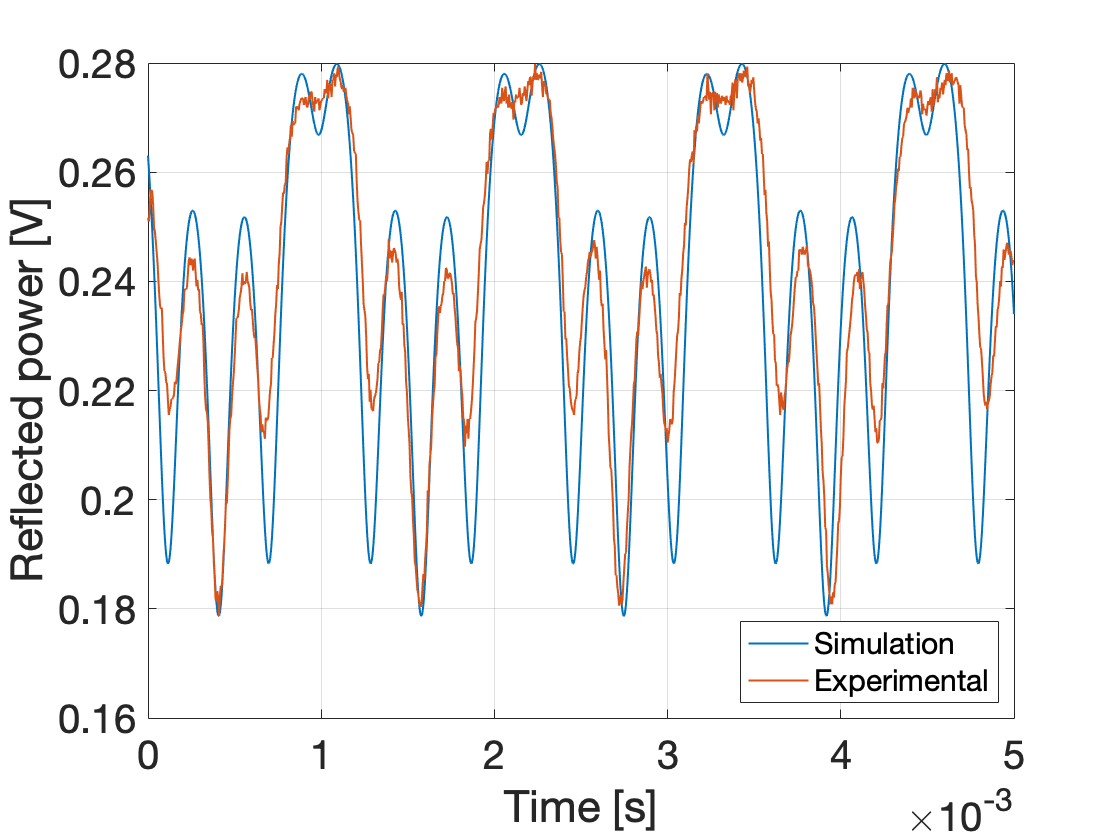
\includegraphics[width=.7\textwidth]{exp-tf-reservoir/tf_25.png}
	\caption{Reflected power [V] as a function of the time [s] during a sweep of the piezo voltage. First sideband halfway between resonance and anti-resonance. $\Omega_{\text{mod}}$ = 19.9997 GHz, modulation depth $m$ = 2, $\gamma = \SI{0.0126}{\per\metre}$. The theoretical curve has been rescaled in order to be compared with the experimental curve.}
	\label{tf_25}
\end{figure}

\paragraph{First sideband at anti-resonance} $\pulsefreq{\omegamod}$ is an odd number of times half of the \gls{fsr}. The graphs are depicted on the figure \ref{tf_50}.\\

\begin{figure}
	\centering
	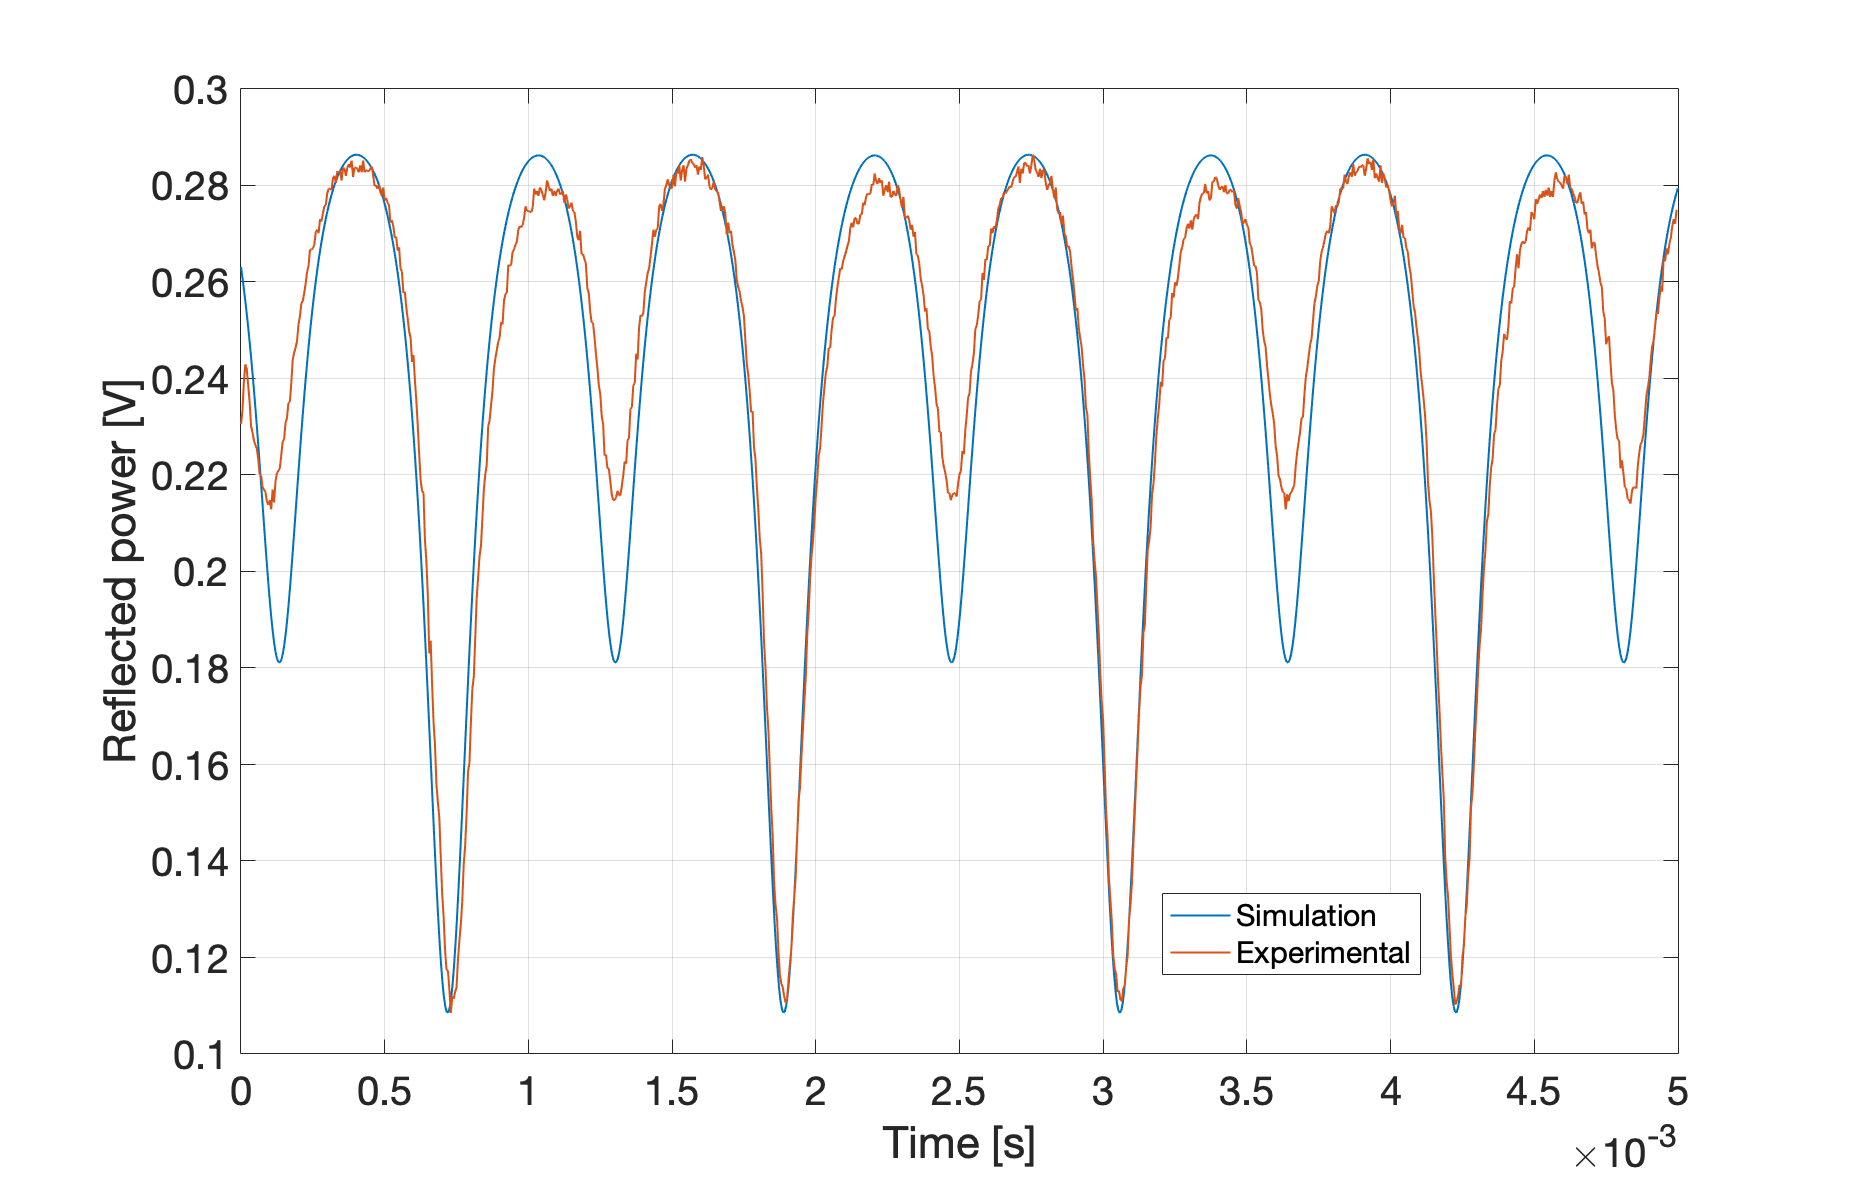
\includegraphics[width=.7\textwidth]{exp-tf-reservoir/tf_50.png}
	\caption{Reflected power [V] as a function of the time [s] during a sweep of the the piezo voltage. First sideband at anti-resonance. $\Omega_{\text{mod}}$ = 19.9997 GHz, modulation depth $m$ = 2, $\gamma = \SI{0.0126}{\per\metre}$. The theoretical curve has been rescaled in order to be compared with the experimental curve.}
	\label{tf_50}
\end{figure}

On those graphs, one can see that the transfer function highly depends on the modulation frequency. Even though the experimental adequacy is not perfect, it is sufficient to have a qualitative idea of the behaviour of the reservoir. It also allows to experimentally deduce its \gls{fsr} by measuring the temporal periodicity of the reflectivity, and then to translate in the frequency domain using equation \eqref{eq-omega-vs-t}.

\begin{equation}
	\Delta t = \SI{1.155}{\milli\second} \Longrightarrow \text{FSR} \approx  \alpha \beta \frac{c}{\lambda_0^2} \Delta t  \approx \SI{11.5}{\mega\hertz}
\end{equation}

Recalling that the \gls{fsr} for a ring cavity is given by:

\begin{equation}
	\mathrm{FSR} = \frac{c}{nL}
\end{equation}

Using this formula, one can compute the length of the cavity: $L=\SI{18.33}{\metre}$.

As a final remark, the relative position of the \gls{pm} inside the cavity (controlled using the variable $\xi$) does not seem to have an influence on the shape of the transfer function.

%%% EFFECTIVE LOSSES %%%

\subsection{Effective losses}

\label{subsec-effective-losses}

Given the model derived, the only physical quantity that cannot be known from a simple inspection of the data sheets are the effective losses $\gamma$. They arise due to the effects of the fibre losses, the insertion loss of the intra-cavity \gls{pm} and the gain of the \gls{edfa}. Their value is determined experimentally. To do so, a least square fit is performed. Basically, this means that one compares an experimental curve with an analytical one, for which the value of $\gamma$ is not fixed. The deviation between those two curves is therefore a function of $\gamma$, and can be minimised. Mathematically speaking, the experimental effective losses $\tilde{\gamma}$ are given by:

\begin{equation}
	\tilde{\gamma} = \underset{\gamma}{\mathrm{argmin}} \sum_{i=1}^T (\mathcal{R}_i - \mathcal{R}(t_i;\gamma))^2
\end{equation}

Where $T$ is the total number samples, $\mathcal{R}_i$ is the measured reflected power for the $i^{\text{th}}$ sample and $\mathcal{R}(t_i;\gamma)$ is the theoretical rescaled reflectivity evaluated at $t=t_i$ and $\gamma$, which is the time corresponding to the $i^{\text{th}}$ sample and the effective losses, respectively. In figure \ref{eff-losses}, one can see the result of this optimisation. It was performed on the reservoir without phase modulation because it is assumed that the insertion losses do not depend on whether a phase modulation is going on. The effective losses that were determined using this procedure read:

\begin{equation}
	\gamma = \SI{0.0126}{\per\metre}
\end{equation}

\begin{figure}
	\centering
	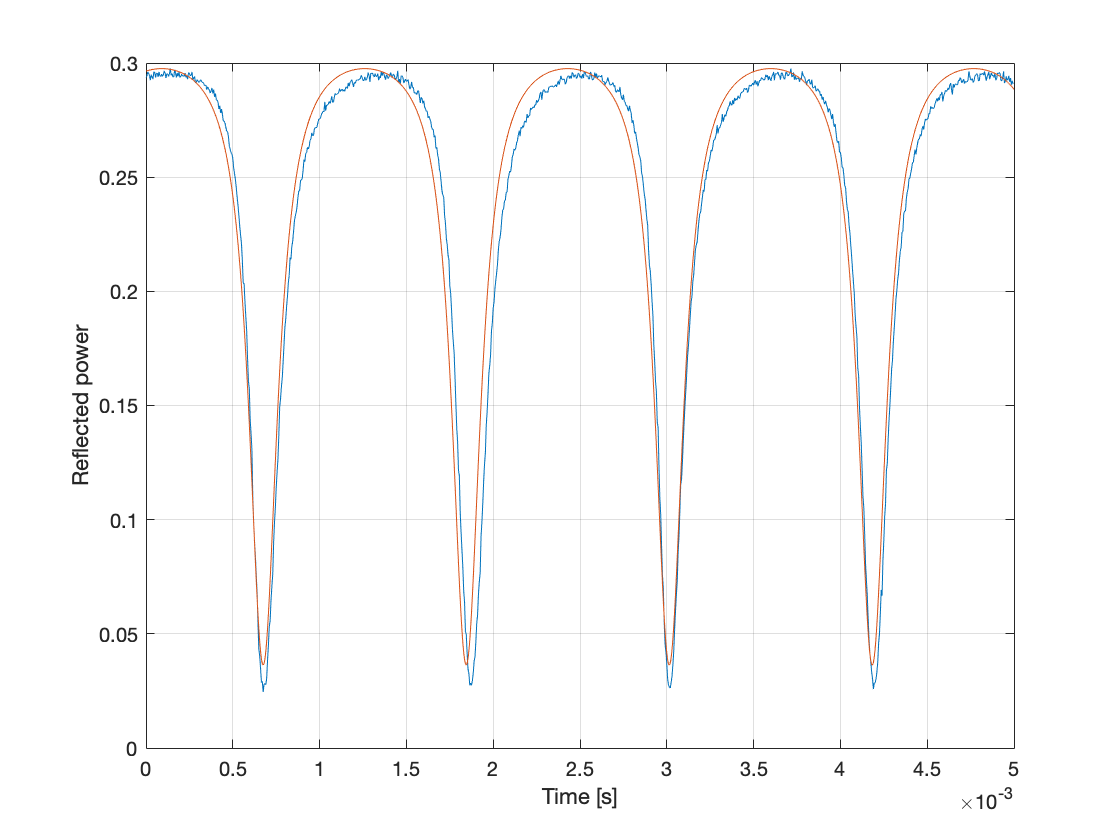
\includegraphics[width=.7\textwidth]{exp-tf-reservoir/eff_losses.png}
	\caption{Reflected power [V] as function of the time [s] during a sweep of the the piezo voltage, no intra-cavity phase modulation, $\gamma = \SI{0.0126}{\per\metre}$. The theoretical curve has been rescaled in order to be compared with the experimental curve.}
	\label{eff-losses}
\end{figure}

%%% MODULATION DEPTH %%%

\subsection{Modulation depth}

When one wants to modify the modulation depth during a phase modulation process, one has to change the modulation power of the RF generator. The goal of this section is to determine an empirical relation linking the modulation power, expressed in dBm, and the modulation depth. The procedure to compute it is the following: one applies a methodology similar to the one from the previous chapter, except that instead of optimising for $\gamma$, one should to do it for $m$, the modulation depth. This procedure is repeated several times, for different modulation powers, in order to form a data set. Finally, when one has gathered enough data, one can perform a polynomial interpolation that provides the link between the power and the depth that one was looking for. This method works better when one is working in the situation where the first sideband is at anti-resonance, because in this this regime, the depth of the side peaks (see figure \ref{tf_50}) depends a lot on the modulation depth.\\

\begin{figure}
	\centering
	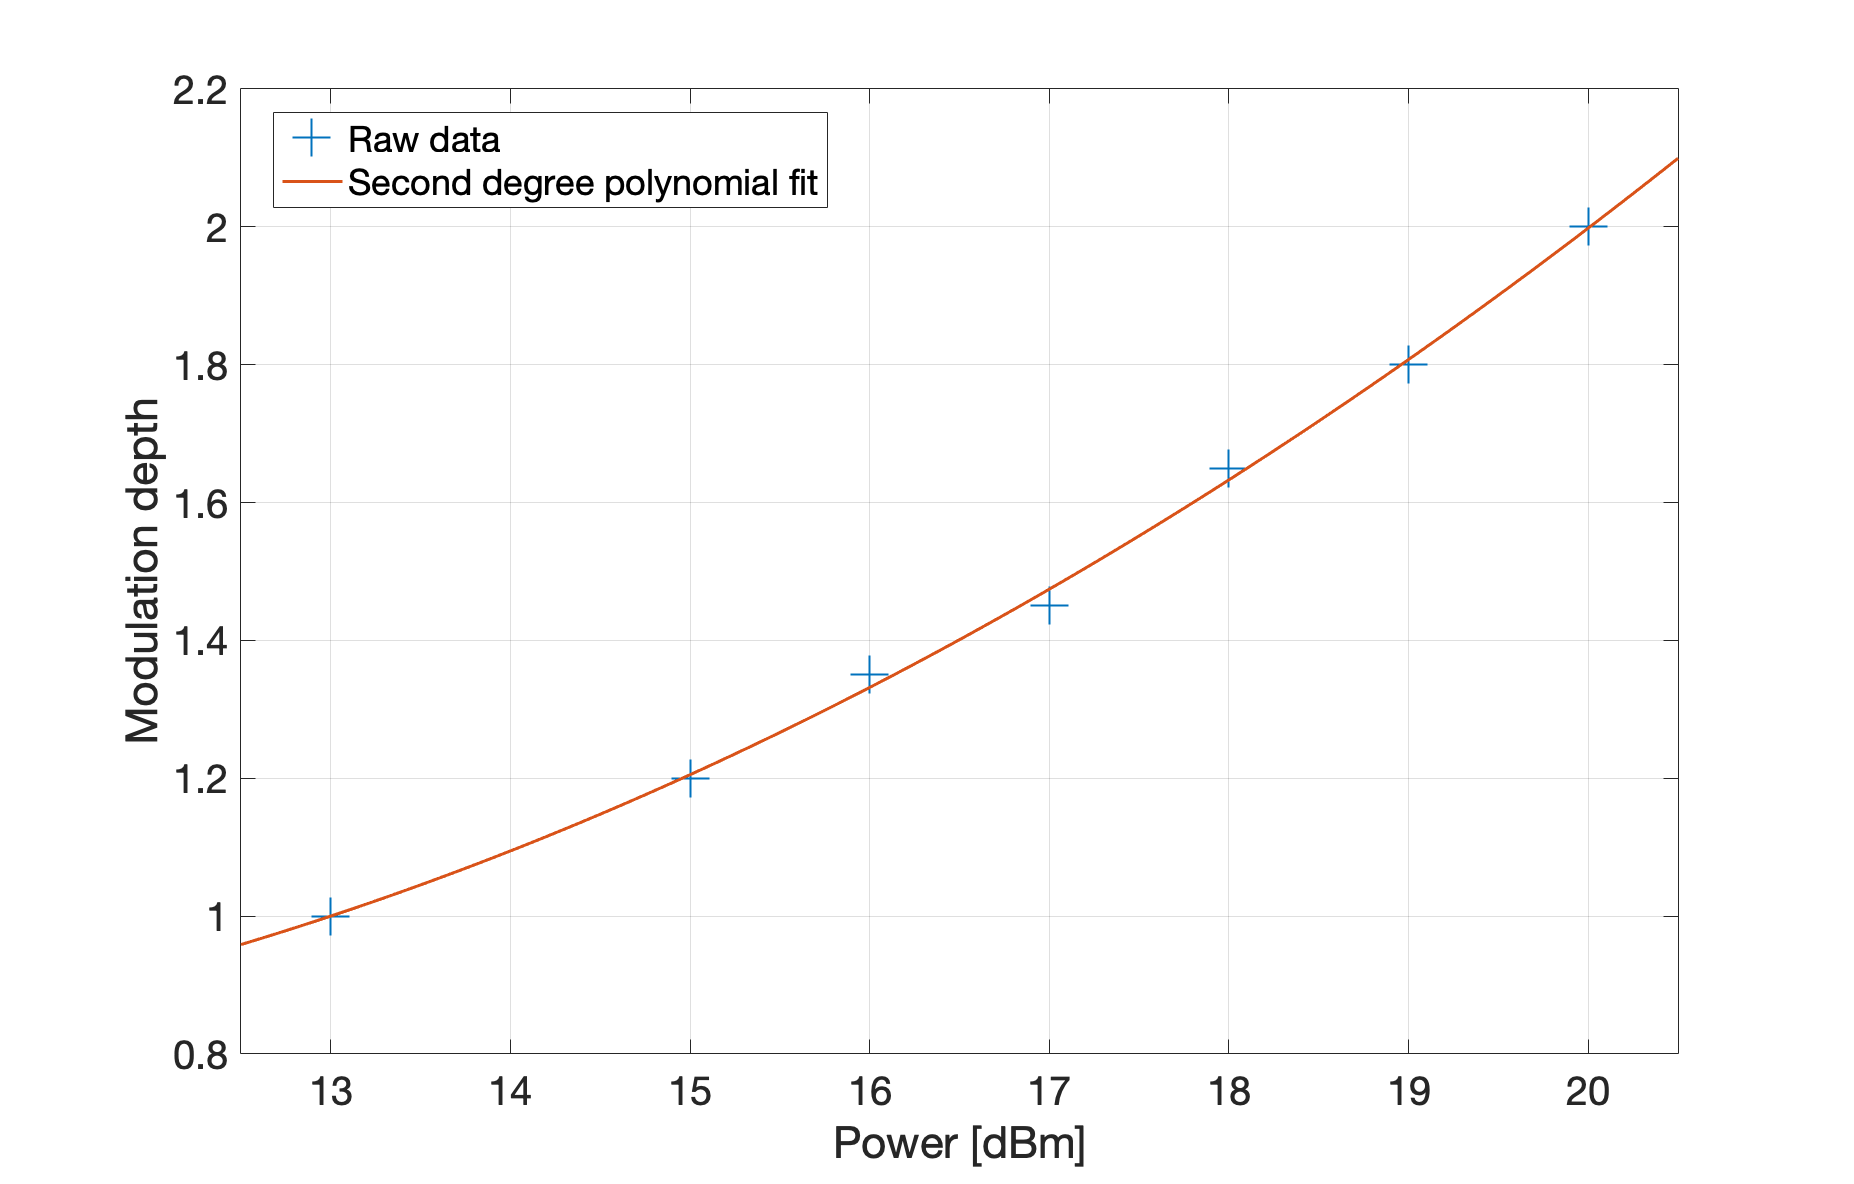
\includegraphics[width=.7\textwidth]{exp-tf-reservoir/mod_depth.png}
	\caption{Modulation depth $m$ as a function of the modulation power [dBm] and second degree polynomial interpolation for $\pulsefreq{\omegamod}=\SI{19.9943}{\giga\hertz}$.}
	\label{mod_depth}
\end{figure}

In figure \ref{mod_depth}, one can see the data, as well as the second degree polynomial interpolation. The experimental points only start at 13 dBm because below this value, the side peak was too small to lead significant measures. As already claimed, one cannot go above $m = 2$ experimentally without external amplification because the RF generator is not able to supply modulation powers higher than 20 dBm at such high modulation frequencies. The empirical polynomial relation is:

\begin{equation}
	m(P[\textrm{dBm}]) = \num{8.004d-3} P^2[\textrm{dBm}] - 0.1215 P[\textrm{dBm}] + 1.222
\end{equation}

It is observed that higher orders can be neglected in the polynomial interpolation.

%%%%%%%%%% PDH STABILISATION TECHNIQUE %%%%%%%%%%

\section{Pound-Drever-Hall stabilisation technique}

\label{sec-pdh}

In this section, the \gls{pdh} stabilisation technique is presented. First, the rationale behind its introduction is discussed. After that, it is shown that the error function resulting from the \gls{pdh} modulation reveals new informations about the phase of the electric field inside the cavity that allow to reach better stabilisation performances. Finally, a few remarks are given regarding the implementation of this scheme for the reservoir cavity.

%%% INTRODUCTION %%%

\subsection{Introduction}

The \gls{pdh} stabilisation technique was proposed in 1983 in \cite{drever1983laser} and since then has proven to be a powerful scheme enabling to accurately stabilise optical cavities. Among other applications, it has been used to to stabilise the laser and measure the thermal noise in the arms of the Michelson interferometer of the LIGO \cite{black1998notes}, which made possible the observation of gravitational waves.\\

The basic idea of the \gls{pdh} technique is to modify the transfer function of the cavity in such a way that its observation will provide more information about the phase. This is implemented in practice by using an additional \gls{pm} and some electronic post-processing, which is handled by the Digilock in our setup.

\subsubsection{Cavity stabilisation}

\label{subsubsec-cavity-stab}

Before discussing the \gls{pdh} scheme, the principles of classical cavity stabilisation are presented. As a reminder, this action consists of keeping the relative phase between the electric field inside the cavity after a round trip and the incident electric field equal to a constant value by maintaining the reflected power equal to the value translating to this relative phase using the transfer function. The reflected power of the cavity is measured using \glspl{pd}, and can be modified by using actuators to change either the length of the cavity, or the emission wavelength of the laser. \\

\begin{figure}
	\centering
	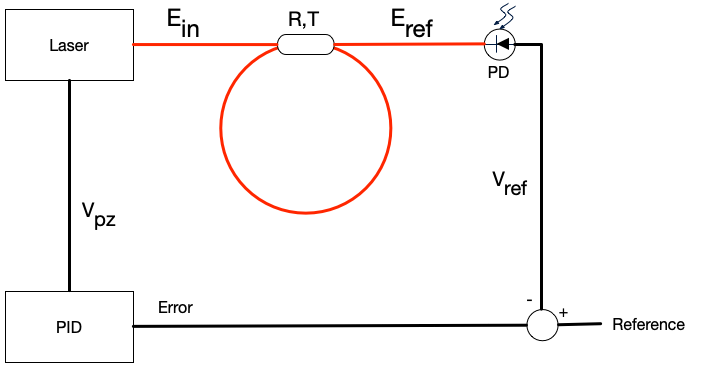
\includegraphics[width=.7\textwidth]{cavity_stab_principle}
	\caption{Schematic representation of a cavity being stabilised using the classical stabilisation technique. The red lines are optical fibres and the black ones are electrical connections.}
	\label{cavity_stab_principle}
\end{figure}

In figure \ref{cavity_stab_principle}, one can observe the basic principle of the regulation of an optical cavity. The top branch of the figure is well-known at this point. The incident field $E_{\text{in}}$ enters the cavity at the level of the coupler, where the reflected $E_{\text{ref}}$ exits the cavity. The latter is then measured by the \gls{pd}. Henceforth, the different elements should be looked at under the light of control theory. The measured voltage $V_{\text{ref}}$ is compared to a reference, which is the value that the regulator is trying to maintain. The difference between the reference and the measured voltage is the so-called error, which is processed by a device named the \gls{pid} regulator. In all generality, a \gls{pid} regulator, or \gls{pid} in short, is governed by this equation in the time domain \cite[p.196]{franklin2015feedback}:

\begin{equation}
	u(t) = k_P e(t) + k_I \int_{-\infty}^t e(\tau) d\tau + k_D \frac{de}{dt}(t)
\end{equation}

With $u(t)$ the output of the \gls{pid}, which is in this context the voltage applied to the piezoelectric $V_{\text{pz}}$, $e(t)$ the error and $k_I$, $k_P$ and $k_D$ the proportional, integral, and differential coefficients, respectively. In order to get the \gls{pid} to work, one needs to tune those three coefficients, either using analytical methods, or heuristically by scanning the different values. The latter option was the one followed in the experimental implementations described in this work.\\

The voltage $V_{\text{pz}}$, the output of the \gls{pid}, is applied to the piezoelectric crystal of the laser and alters its emission wavelength to stay synchronised with the reference.\\

The main limitation of this scheme is linked to the symmetry of the transfer function $\mathcal{R}$. Let us illustrate why the symmetry is a shortcoming by considering a specific situation, with the help of the figure \ref{tf_near_resonance}.  Let us assume an initial condition when one has a cavity stabilised at the resonance, namely at the minimum of the curve. If the cavity is disturbed by any kind of perturbations, the reflected signal will increase, but due to the symmetry with respect to the resonance frequency, how will one know if the phase is increasing or decreasing ? The measured signal will be exactly the same in both situations. This is problematic because instead of rejecting the perturbations, the \gls{pid} could amplify them by interpreting the measured signal in the wrong way. A trick to still be able to stabilise a cavity using this method is to consider not only the instantaneous value of the reflected signal, but also its slope. Doing so, one is able to differentiate between a larger (positive slope) or smaller (negative slope) frequency. Yet, this workaround is not recommended because it is more convenient to work only with instantaneous signals. The \gls{pdh} technique overcomes this limitation by introducing a transfer function, called the error function, which is antisymmetric with respect to the resonance frequencies.

\begin{figure}
	\centering
	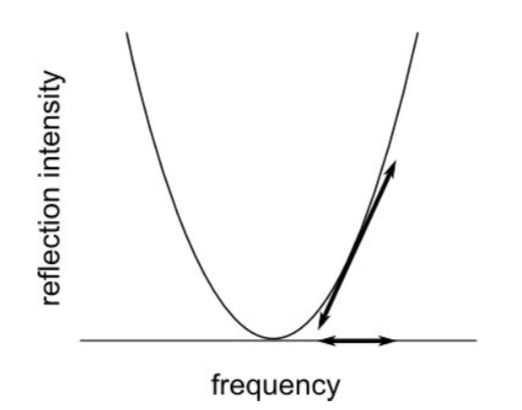
\includegraphics[width=.5\textwidth]{tf_near_resonance}
	\caption{Schematic graph of the transfer function $\mathcal{R}$ near a resonance as function of the frequency \cite{nickersonreview}.}
	\label{tf_near_resonance}
\end{figure}

%%% PDH SCHEME %%%

\subsection{Pound-Drever-Hall scheme}

\label{subsec-pdh-technique}

\begin{figure}[h]
	\centering
	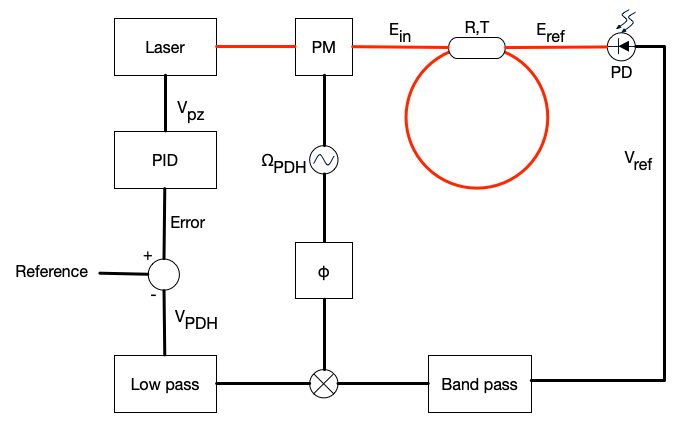
\includegraphics[width=.7\textwidth]{pdh_principle}
	\caption{Schematic representation of a cavity being stabilised using the \pdh technique. This schematic is based on the original blueprint presented in \cite{drever1983laser}. The colour convention for the lines is the same as in the previous figures. The phase of the light incident on the cavity is modulated by a \gls{pm} driven by a local oscillator. The reflected power undergoes a band pass filtering, a mixing with the signal of the local oscillator shifted by a phase $\phi$ and a low pass filtering. The \pdh error function is denoted by $\tind{V}{PDH}$. It is compared to a reference level to provide an error signal to the \gls{pid}.}
	\label{pdh_principle}
\end{figure}

The \gls{pdh} stabilisation technique relies on the addition of a \gls{pm} and electronic post-processing, as can be viewed in figure \ref{pdh_principle}. The light sent by the laser goes through a \gls{pm} driven by an AC voltage at frequency $\pulsefreq{\tind{\Omega}{PDH}}$ emitted by a RF generator. The modulation depth is chosen in such a way that all the sidebands but the first are negligible (one sideband on each side of the carrier frequency). Therefore, the electric field incident on the cavity $\tind{E}{in}$ reads:

\begin{equation}
	\tind{E}{in} = E_0 \left(J_0(m) e^{i\omega t} + J_1(m)e^{i(\omega +\tind{\omega}{PDH})t} - J_1(m)e^{i(\omega -\tind{\omega}{PDH})t}  \right)
\end{equation}

Given the fact that the cavity is linear, one can assume that its transfer function\footnote{As a reminder, the transfer function is the function such that $|R|^2=\mathcal{R}$} $R$ is linear as well, which gives for the reflected field $\tind{E}{ref}$:

\begin{gather}
	\tind{E}{ref} = E_0 ( J_0(m) R(\omega) \phaseone{\omega} + J_1(m) R(\omega+\tind{\Omega}{PDH}) \phase{\omega+\tind{\Omega}{PDH}} \nonumber \\
	- J_1(m) R(\omega-\tind{\Omega}{PDH}) \phase{\omega-\tind{\Omega}{PDH}} )
\end{gather}

The voltage at the \gls{pd} is proportional to the intensity:

\begin{gather}
	\tind{V}{ref} \propto |E_0|^2 \bigg( J_0^2(m) \mathcal{R}(\omega) + J_1^2(m) (\mathcal{R}(\omega+\tind{\Omega}{PDH}) + \mathcal{R}(\omega-\tind{\Omega}{PDH})) \nonumber \\
	+ 2 J_0(m)J_1(m) \text{Re}[R(\omega)R^*(\omega+\tind{\Omega}{PDH})-R^*(\omega)R(\omega-\tind{\Omega}{PDH})] \cos{(\tind{\Omega}{PDH} t)} \nonumber \\
	+ 2 J_0(m)J_1(m) \text{Im}[R(\omega)R^*(\omega+\tind{\Omega}{PDH})-R^*(\omega)R(\omega-\tind{\Omega}{PDH})] \sin{(\tind{\Omega}{PDH} t)} \nonumber \\
	+ \text{terms at } 2\tind{\Omega}{PDH} \bigg)
\end{gather}

This signal goes to a band pass filter centred at $\tind{\Omega}{PDH}$ in order to remove the DC component and the terms oscillating at $2\tind{\Omega}{PDH}$. Let us define $\zeta(\omega)$ as:

\begin{equation}
	\zeta(\omega) = R(\omega)R^*(\omega+\tind{\Omega}{PDH})-R^*(\omega)R(\omega-\tind{\Omega}{PDH})
\end{equation}

The voltage at the output of the band pass filter reads:

\begin{equation}
	\tind{V}{BP} \propto \text{Re}[\zeta(\omega)]\cos{(\tind{\Omega}{PDH}t)} + \text{Im}[\zeta(\omega)] \sin{(\tind{\Omega}{PDH}t)}
\end{equation}

After that, the signal is mixed with the local oscillator driving the \gls{pm}, shifted by an additional phase $\phi$. A mixer is basically a nonlinear electronic device that multiplies two signals. Multiplying $\tind{V}{BP}$ by $\sin{(\tind{\Omega}{PDH}t+\phi)}$ leads to a DC component, which contains the information one is trying to extract, and to a $2\tind{\Omega}{PDH}$ component. At this point, one only has to use a low pass filter to retrieve the signal \cite{nickersonreview}. Recalling two trigonometric identities:

\begin{align}
	\cos{(\tind{\Omega}{PDH}t)}\cdot \sin{(\tind{\Omega}{PDH}t+\phi)} &= \frac{1}{2} (\cos{(2\tind{\Omega}{PDH}t+\phi)}+\sin{(\phi)})  \\
	\sin{(\tind{\Omega}{PDH}t)}\cdot \sin{(\tind{\Omega}{PDH}t+\phi)} &= \frac{1}{2} (-\cos{(2\tind{\Omega}{PDH}t+\phi)}+\cos{(\phi)}) 
\end{align}

One can see that multiplying $\tind{V}{BP}$ by $\sin{(\tind{\Omega}{PDH}t+\phi)}$ and then low pass filtering yields to the following expression for $\tind{V}{PDH}$:

\begin{equation}
	\tind{V}{PDH} \propto \text{Re}[\zeta(\omega)]\sin{(\phi)} + \text{Im}[\zeta(\omega)]\cos{(\phi)}
\end{equation}

One can therefore select which component to use by changing the value of $\phi$. The \gls{pdh} error function $\varepsilon(\omega)$ is defined as:

\begin{equation}
	\varepsilon(\omega) = \text{Im}[\zeta(\omega)]
\end{equation}

The graph of the \gls{pdh} error function is depicted on the right side of figure \ref{im_zeta}. As required, it is antisymmetric with respect to the resonance frequency, which allows to immediately differentiate between an increase or a decrease of phase. Moreover, thanks to the steep slope of the curve at resonance, a small variation of phase implies a large variation of $\varepsilon$. On the right side of the figure, one can see that $\text{Re}[\zeta]$ provides no useful information about the phase, which is why it is not used in practice.\\

The end of the regulation scheme is the same as the previous one. The \gls{pdh} signal $\tind{V}{PDH}$ (with $\phi=0$) is compared to a reference, which gives the error, and this error is used by the \gls{pid} to regulate the laser. This scheme can stabilise the cavity at any phase, provided that the slope on the neighbourhood of this phase is steep enough. This condition being quite vague, it should be checked experimentally whether it is possible to stabilise at a given phase.\\

\begin{figure}[h]
	\centering
	\begin{subfigure}{.5\textwidth}
		\centering
		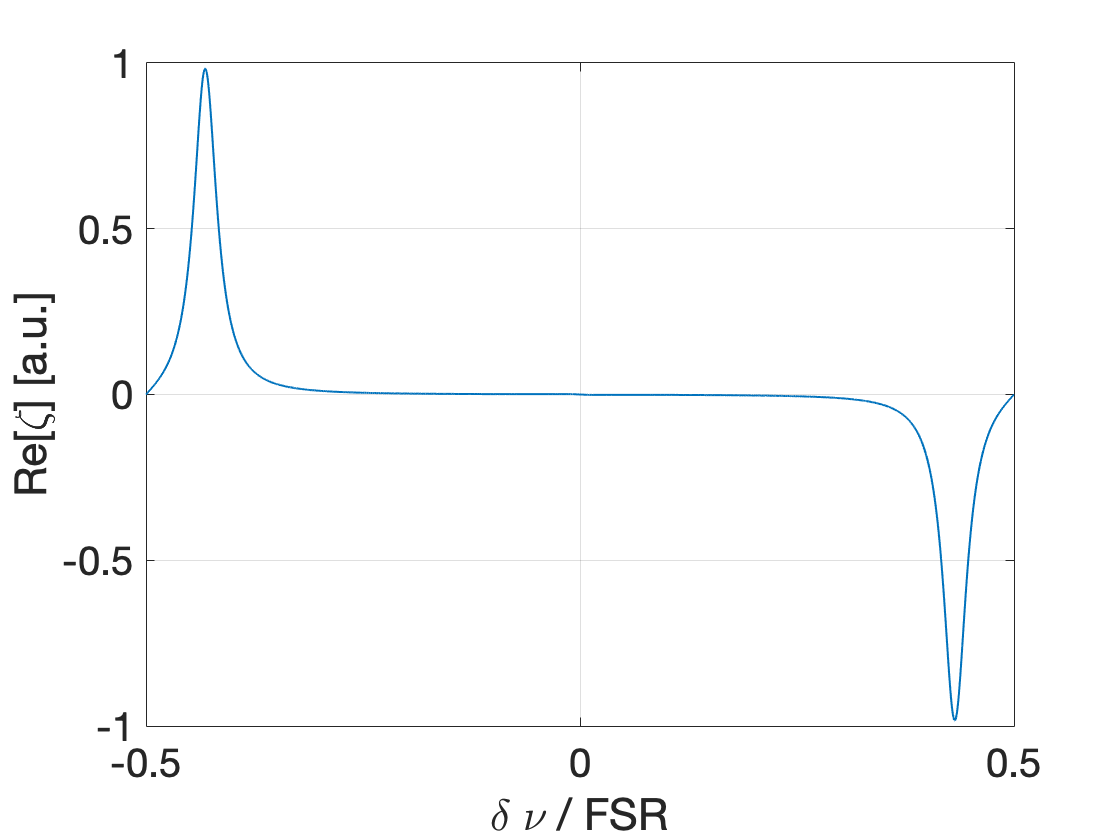
\includegraphics[width=\textwidth]{pdh_th/re_zeta.png}
	\end{subfigure}%
	\begin{subfigure}{.5\textwidth}
		\centering
		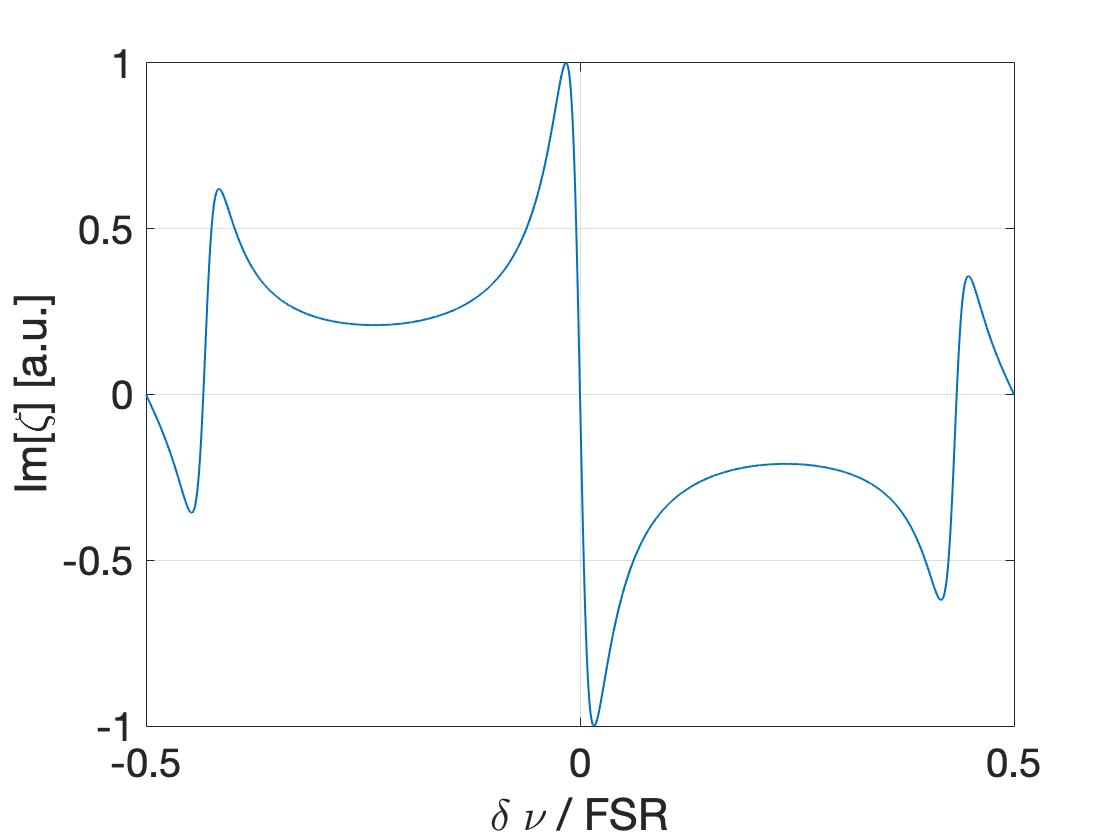
\includegraphics[width=\textwidth]{pdh_th/im_zeta.png}
	\end{subfigure}
	\caption{Normalised $\text{Re}[\zeta]$ (left) and normalised \pdh error function $\epsilon$ (right) as a function of the normalised frequency $\delta \nu / \text{FSR}$ for a ring cavity with $\pulsefreq{\tind{\Omega}{PDH}}=\SI{58}{\percent}$ of the \gls{fsr}.}
	\label{zeta}
\end{figure}

%%% PDH TECHNIQUE FOR THE RESERVOIR %%%

\subsection{Pound-Drever-Hall technique for the reservoir}

The \gls{pdh} technique can be applied to stabilise the reservoir, but error needs to be slightly modified to take into account the presence of different wavelengths inside the cavity. The result is actually quite straightforward if one recalls the results from section \ref{subsubsec-tf-cavity}. The reflected field is simply given by $\efield{ref} = E_0 \sum_{n=-\eta}^\eta R_{n,0}(\omega) \hat{\mathbf{e}}_n$ thanks to the reservoir transfer matrix $\mathbf{R}$ given by equation \eqref{eq-tf-matrix} and that the \gls{pd} cannot capture beatings whose frequencies are integer multiples of \SI{20}{\giga\hertz}. With these two elements in mind, $\zeta(\omega)$ becomes:

\begin{equation}
	\zeta(\omega) = \sum_{n=-\eta}^\eta R_{n,0}(\omega)R_{n,0}^*(\omega+\tind{\Omega}{PDH}) - R_{n,0}^*(\omega) R_{n,0}(\omega - \tind{\Omega}{PDH})
\end{equation}

The error function $\epsilon$ remains defined as the imaginary part of $\zeta$. In figure \ref{pdh_exp}, one can observe that the theoretical model is in line with the measured error function. Just like the reflectivity of the reservoir $\mathcal{R}$, the shape of the \pdh error function depends on the intra-cavity modulation frequency. The graph does not have the same shape as the one from figure \ref{zeta}, but since it exhibits regions with steep slopes, it can be used to stabilise the reservoir. In practice, the Digilock handles all the data-processing that has been introduced in this section, and the \gls{pid} regulation as well.

\begin{figure}
	\centering
	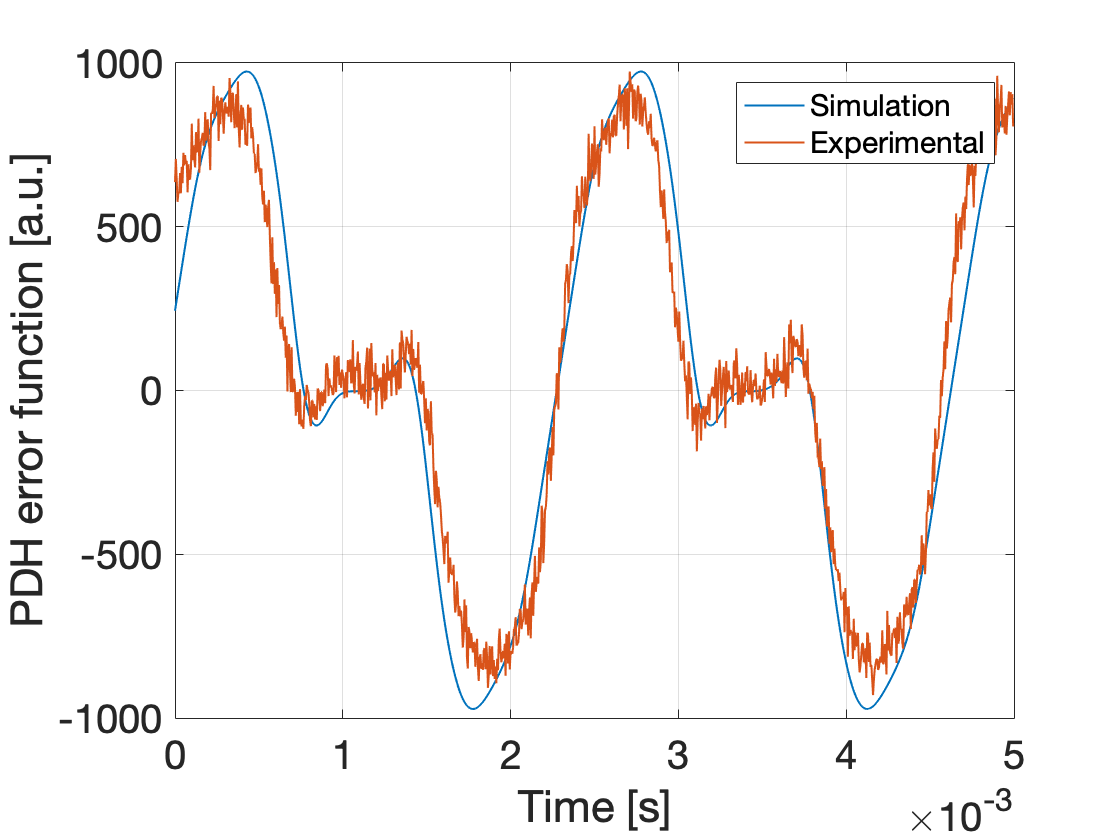
\includegraphics[width=.7\textwidth]{pdh_exp/3130_4.png}
	\caption{\gls{pdh} error signal $\epsilon$ as a function of the time [s] for the reservoir cavity during a sweep of the Digilock. \gls{pdh} Modulation amplitude $\tind{V}{PDH}= \SI{0.4}{\voltptp}$ (peak to peak), \gls{pdh} modulation frequency $\tind{\nu}{PDH} = \SI{3.13}{\mega\hertz}$, intra-cavity modulation depth $m=2$, intra-cavity modulation frequency $\tind{\nu}{mod} = \SI{19.9998}{\giga\hertz}$. The theoretical curve has been rescaled in order to be compared with the experimental curve.}
	\label{pdh_exp}
\end{figure}

%%%%%%%%%% CHARACTERISATION OF THE STABILISATION PERFORMANCE FOR DIFFERENT REGIMES %%%%%%%%%%

\section{Characterisation of the stabilisation performance for different regimes}

This section presents the performances that can be achieved when stabilising the reservoir with the help of the \gls{pdh} scheme, which is the core issue tackled in this thesis. First, the problem is recalled and specified in a comprehensive way, then the experimental procedure followed to obtain relevant data is presented, and finally the actual results are shown and discussed.

As already claimed, the \gls{pdh} technique is capable of stabilising the cavity at any phase, provided that the slope of the \gls{pdh} error function is steep enough for this phase. Therefore, one the features being investigated experimentally is the determination of the range of phases at which the cavity can be stabilised. This is of great practical importance, because as shown in section \ref{model-reservoir}, the phase accumulated at each round trip is a global parameter that can alter the performances of the \rcer.\\

Another element that has been studied experimentally is the quality of the stabilisation. First, one has to use a relevant metric to assess how good the reservoir is stabilised. What is used throughout this section is the standard deviation of the phase during one run of measurements. Assume one is stabilising the reservoir at phase $\phi$ for some time. The phase inevitably fluctuates, but the better the cavity is stabilised, the lower these fluctuations. By recording the change of the phase, one can compute the standard deviation, the so-called phase noise, which therefore gives a quantitative indication on the efficiency of the stabilisation. This estimation can be done based on different kinds of signals, as it is explained in section \ref{subsec-approach}.\\

The \gls{pdh} technique also has its drawbacks. The phase modulation required to break the symmetry exhibited by the transfer function of the reservoir induces oscillations in the incident electric field, and therefore on the reflected power. The amplitude of these oscillations is mostly dependent on the \gls{pdh} modulation amplitude and can be detrimental to the performances of the \rcer. Intuitively, one can understand that if $\tind{A}{PDH}$ is increased, this will result in larger oscillations, which is problematic because in general, boosting the modulation amplitude allows to obtain a sharper \gls{pdh} error function, with a better \gls{snr}, ultimately enabling to reach a more robust stabilisation. A trade-off has to found between a high-performance stabilisation scheme and low \pdh phase modulation aplitude, as one does not want to improve one feature at the cost of completely deteriorating the other.\\

These different issues are investigated for different \gls{pdh} phase modulation regimes, namely couple of values of $\tind{A}{PDH}$ and $\tind{\Omega}{PDH}$. At the end of the day, this thorough characterisation of the stabilisation properties of the reservoir allows one to choose the regulation parameters that lead to the best chance of making the \rcer work.

%%% APPROACH %%%

\subsection{Approach}

\label{subsec-approach}

Before explaining the experimental procedure, a few points have to be discussed. First, compared to an actual \rcer experiment, the characterisation procedure is simplified because the amplitude of the electric field is not modulated by the \gls{mzm}. As a reminder, during an \rcer experiment, the light source driving the cavity has to be modulated in intensity to carry te data to be processed. In practice, the intensity modulation deteriorates the stabilisation signals, and this will need to be taken into account in the future, yet it has been neglected in the present analysis because not all challenges can be tackled at the same time. What is assumed, however, is that the \gls{pdh} regime allowing to reach the best stabilisation is the same regardless of the intensity modulation being active or not.\\

To avoid any confusion, let us introduce the terminology used in this section:

\begin{itemize}
	\item Transfer function: this is the transfer function of the cavity $\mathcal{R}$ (time-independent)
	\item Reflected power: this is the power reflected by the reservoir (time-dependent)
	\item Error function: this is the \gls{pdh} error function of the cavity $\epsilon$ (time-independent)
	\item Error signal: this is the instantaneous \gls{pdh} error (time-dependent)
\end{itemize}

As far as the experimental parameters are concerned, preliminary numerical simulations\footnote{Courtesy to Lorenz Butschek} showed that \rcer tends to exhibit better performances when $\tind{\nu}{mod}$ is close to, but not exactly, an integer number of times the \gls{fsr}. Therefore, the intra-cavity modulation was chosen with $\tind{\nu}{mod} = \SI{19.9998}{\giga\hertz}$, and with a modulation power $\tind{P}{mod} = \SI{20}{\dbm}$ ($m=2$). This modulation frequency is obtained by taking the one at which the first sideband is at resonance detuned by \SI{500}{\kilo\hertz}. It is therefore important to note that all the results of this section will only be valid for this modulation frequency, since changing it completely modifies the transfer and error functions of the reservoir. The characterisation covers different \gls{pdh} regimes: the modulation frequency $\tind{\nu}{PDH}$ take the values \SI{390}{\kilo\hertz}, \SI{781}{\kilo\hertz}, \SI{1.56}{\mega\hertz} and \SI{3.13}{\mega\hertz} and the modulation amplitude $\tind{V}{PDH}$ \SI{0.2}{\voltptp}, \SI{0.3}{\voltptp} and \SI{0.4}{\voltptp}. For all the frequencies, the three voltages are investigated except for $\tind{\nu}{PDH} = \SI{390}{\kilo\hertz}$ where only $\tind{V}{PDH} = \SI{0.4}{\voltptp}$ is studied. A peculiarity of the regulation for the reservoir is that the proportional and derivative terms of the \gls{pid} have no influence on the stabilisation. At this point, there is no clear explanation on why it is the case, but performing a proper characterisation of the step responses of all the devices involved in the regulation could bring some insight. Furthermore, the impact of the value of $k_I$, the integral coefficient on the \gls{pid}, on the stabilisation is very limited. Several order of magnitude can be spanned without altering significantly the quality of the regulation. The coefficient was set heuristically to $k_I=\SI{17000}{\volt\per\second}$ because around this value the results seemed better, and was kept constant for all the measurements.\\

In the following paragraphs, the different quantities experimentally studied are presented, and the methodology followed to compute is explained.

% PHASE %

\subsubsection{Phase}

\begin{figure}[h]
	\centering
	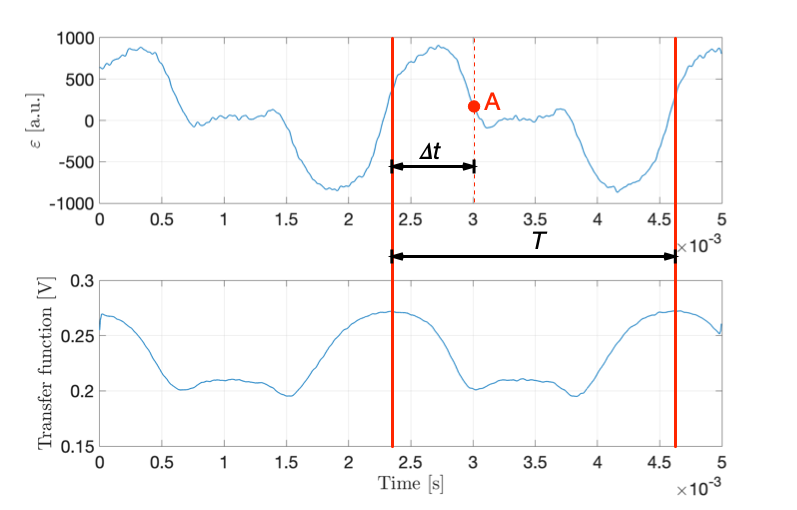
\includegraphics[width=.7\textwidth]{stab_phase/phase.png}
	\caption{Error function [a.u.] and transfer function [\si{\volt}] as a function of the time [\si{\second}] with $\tind{A}{PDH} = \SI{0.4}{\voltptp}$ and $\tind{\nu}{PDH} = \SI{3.13}{\mega\hertz}$, and schematic representation of the method followed to compute the phase. The point $A$ is the point at which the reservoir is stabilised. $T$ is the time taken during a sweep to go over two anti-resonances. $\Delta t$ is the delay separating the $x$-coordinate of $A$ from the first anti-resonance.}
	\label{phase}
\end{figure}

The first key feature to determine is the phase at which one is stabilising. In practice, to choose the stabilisation position, a \gls{pdh} error signal level is selected as reference using the Digilock. To relate the \gls{pdh} error signal value to a phase, one needs to use both the error signal and the transfer function, as depicted in figure \ref{phase}. The transfer function is used to determine the position of the anti-resonance, located at the maxima, which corresponds to a phase of $\pm \SI{\pi/2}{\radian}$. Let $A\equiv(t^*,\epsilon^*)$ be the point whose $y$-coordinate corresponds to the reference error function value $\epsilon^*$ set up in the Digilock. If $T$ is the delay between two maxima of the transfer function, and if $\Delta t$ is the time interval between $t^*$ and the first maximum, then the phase is given by:

\begin{equation}
	\phi = -\frac{\pi}{2} + \frac{\Delta t}{T} \pi
\end{equation}

Let the region of the \gls{pdh} error function comprised between the two maxima of the transfer function be the restricted error function. For a given \pdh error function value $\epsilon^*$, if there exists several points $B\equiv (t,\epsilon^*)$ in the restricted region, then it might be possible to stabilise at this value $\epsilon^*$, but it will be impossible to infer the corresponding phase.

% PDH SIGNAL %

\subsubsection{Pound-Drever-Hall signal}

\begin{figure}
	\centering
	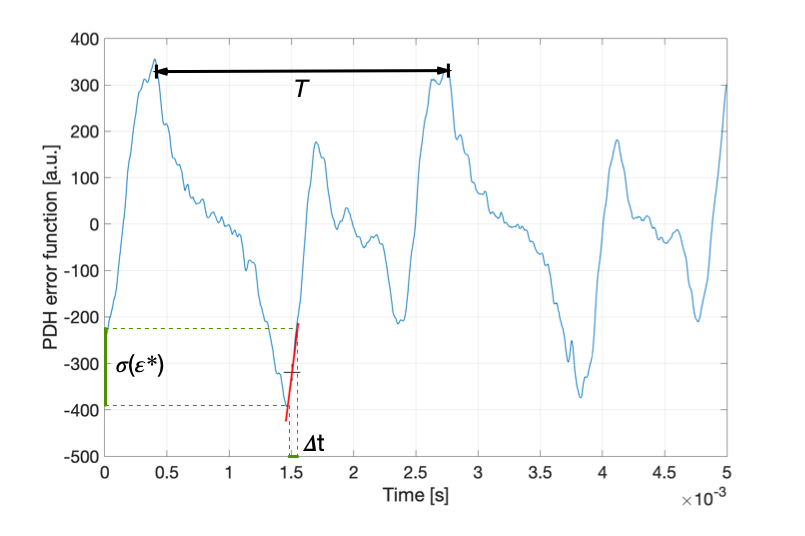
\includegraphics[width=.7\textwidth]{stab_pdh/error_function.png}
	\caption{Error function as a function of the time [\si{\second}] with $\tind{A}{PDH} = \SI{0.4}{\voltptp}$ and $\tind{\nu}{PDH} = \SI{390}{\kilo\hertz}$, reservoir stabilised at $\epsilon^* = \SI{-300}{\au}$. Error signal for this stabilisation is represented in figure \ref{stab_pdh_signal}.}
	\label{stab_prdh_error_function}
\end{figure}

\begin{figure}
	\centering
	\includegraphics[width=.7\textwidth]{stab_pdh/signal.png}
	\caption{Error signal as a function of the time [\si{\second}] with $\tind{A}{PDH} = \SI{0.4}{\voltptp}$ and $\tind{\nu}{PDH} = \SI{390}{\kilo\hertz}$, reservoir stabilised at $\epsilon^* = \SI{-300}{\au}$. The experimental conditions are the same as in \ref{stab_prdh_error_function}.}
	\label{stab_pdh_signal}
\end{figure}

The next value of interest is the phase noise estimated based on the error signal. On the figure \ref{stab_pdh_signal}, one can see the evolution of the \pdh error signal when the reservoir is being stabilised at \SI{-300}{\au}. Based on these data, one can easily compute the standard deviation of the error signal $\sigma(\epsilon^*)$. This value still needs to be translated into a phase noise. To do so, one uses the error function displayed on the figure \ref{stab_prdh_error_function}. First, one linearises the error function at the point of interest, which is represented by the red line segment on the figure. This allows to locally link $\sigma(\epsilon^*)$ to a time variation $\Delta t$. Because the relation linking the wavelength of the laser to the piezo voltage is proportional, the ratio between $\Delta t$ and $T$ (the delay between two maxima, as previously) is the same as the ratio between $\tind{\sigma}{PDH}$, the phase noise in \si{\radian}, and $\pi$. If one defines $\alpha$ as the slope of the tangent at the point of interest (in \si{\au\per\second}), the phase noise reads:

\begin{equation}
	\tind{\sigma}{PDH} = \frac{\tind{\sigma(\epsilon^*)}{PDH} }{|\alpha| T} \pi
\end{equation}

This justify why it is better to work with steep slopes when using the \pdh technique.

% REFLECTED POWER %

\subsubsection{Reflected power}

\begin{figure}
	\centering
	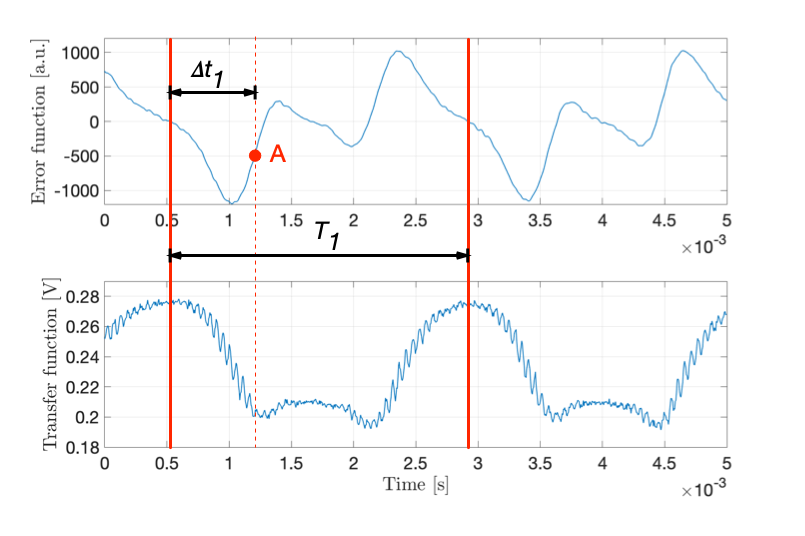
\includegraphics[width=.7\textwidth]{stab_ref/stab_pdh_tf.png}
	\caption{Error function and transfer function [\si{\volt}] as a function of the time [\si{\second}], with $\tind{A}{PDH} = \SI{0.4}{\voltptp}$ and $\tind{\nu}{PDH} = \SI{781}{\kilo\hertz}$, and with the reservoir stabilised at $\epsilon^* = \SI{-500}{\au}$. The reflected power for this stabilisation is illustrated in figure \ref{stab_ref_reflected}.}
	\label{stab_ref_pdh_tf}
\end{figure}

\begin{figure}
	\centering
	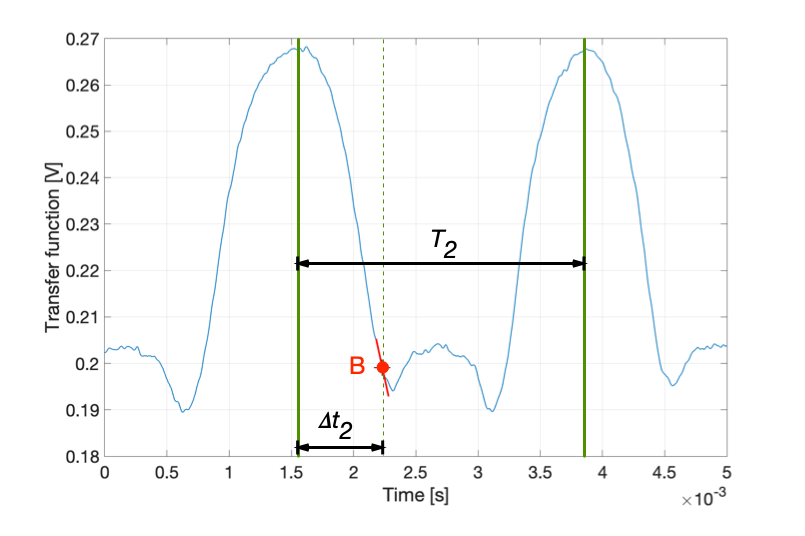
\includegraphics[width=.7\textwidth]{stab_ref/tf.png}
	\caption{Transfer function [\si{\volt}] as a function of the time [\si{\second}] without \pdh modulation, with the reservoir stabilised at $\epsilon^* = \SI{-500}{\au}$. It is the same transfer function as in figure \ref{stab_ref_pdh_tf}, except that there is no phase modulation to be able to compute the slope at the point $B$. The point $B$ corresponds to the same stabilisation position than the point $A$ in figure \ref{stab_ref_pdh_tf}. The $x$-coordinate of $B$ reads $\Delta t_2 = \frac{\Delta t_1}{T_1}T_2$. The reflected power for this stabilisation is illustrated in figure \ref{stab_ref_reflected}.}
	\label{stab_ref_tf}
\end{figure}

\begin{figure}
	\centering
	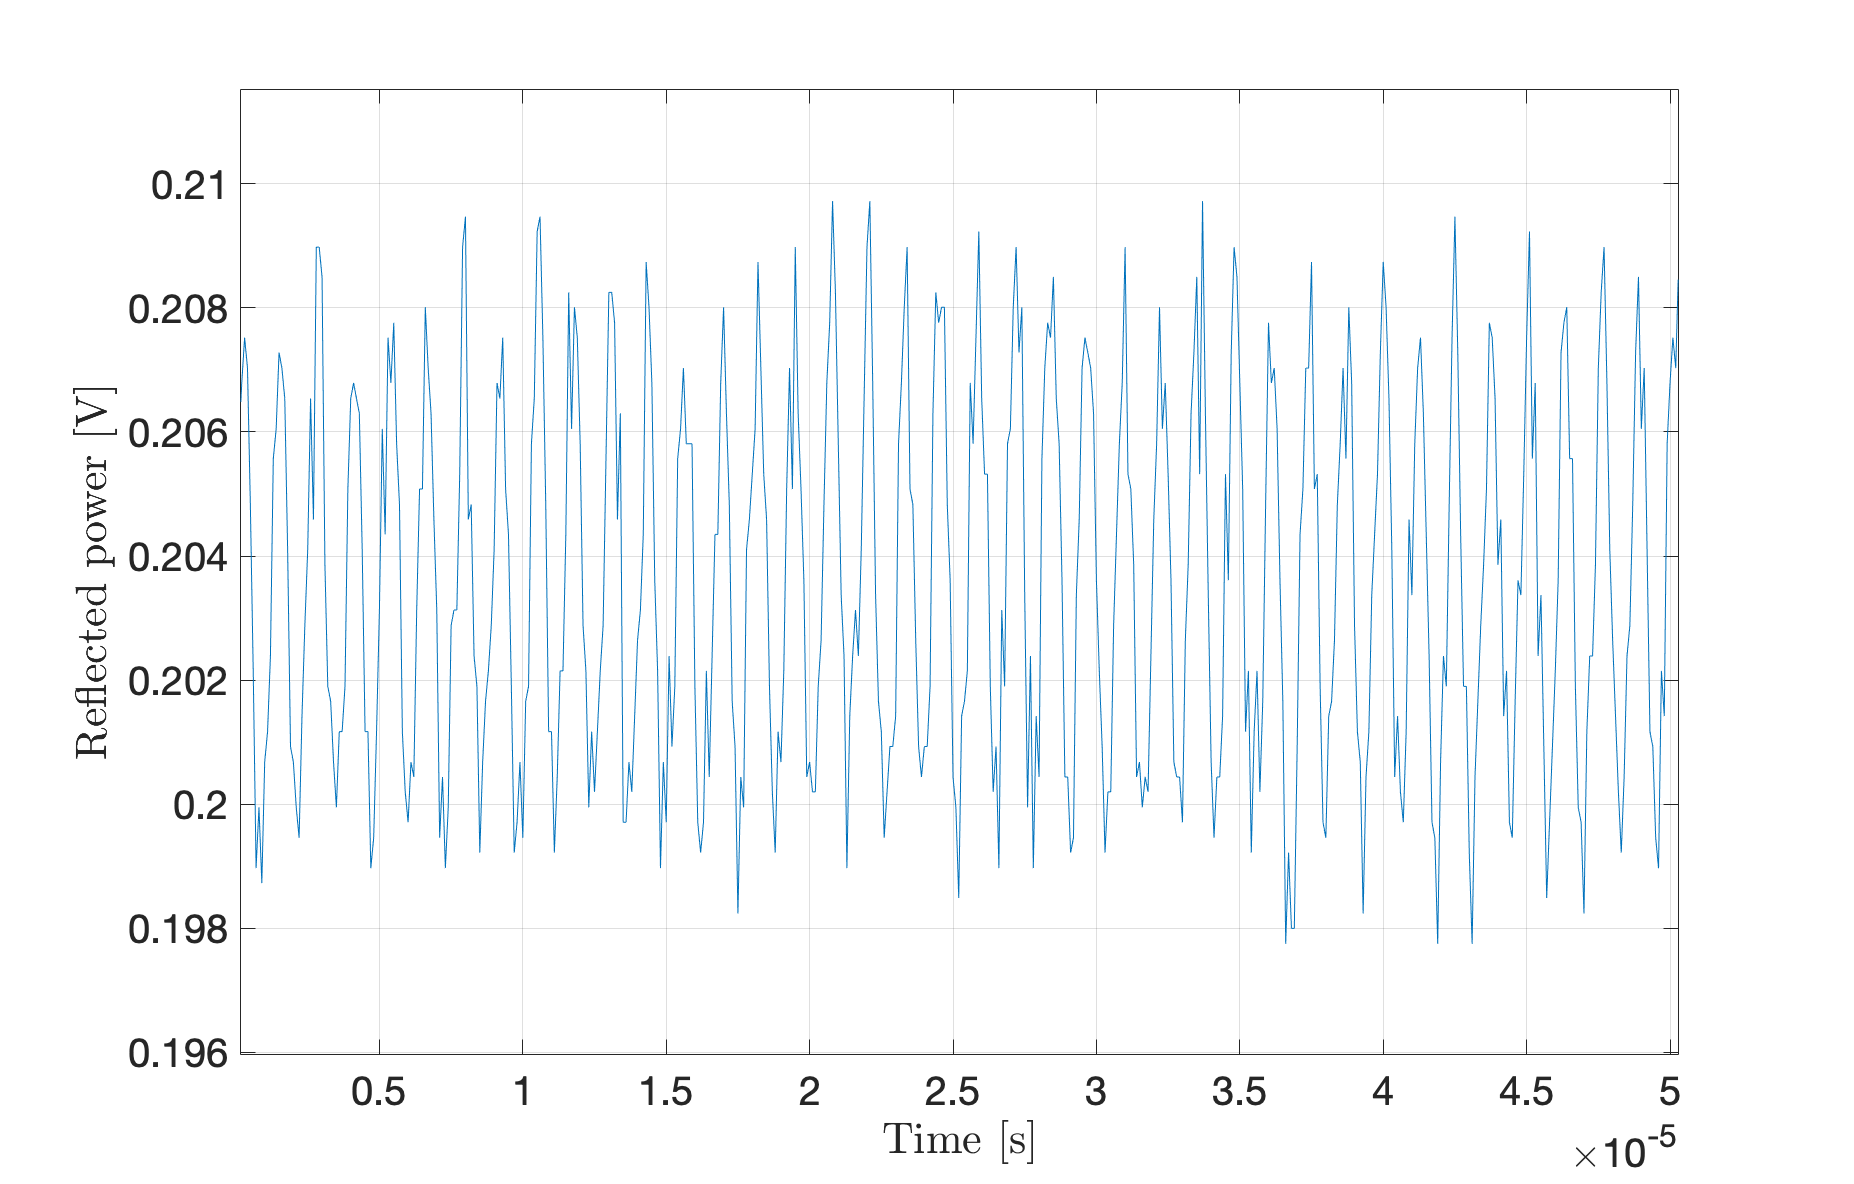
\includegraphics[width=.7\textwidth]{stab_ref/reflected.png}
	\caption{Reflected power [\si{\volt}] as a function of the time [\si{\second}] with $\tind{A}{PDH} = \SI{0.4}{\voltptp}$ and $\tind{\nu}{PDH} = \SI{781}{\kilo\hertz}$ and with the reservoir stabilised at $\epsilon^* = \SI{-500}{\au}$. The experimental conditions are the same as in figures \ref{stab_ref_pdh_tf} and \ref{stab_ref_tf}.}
	\label{stab_ref_reflected}
\end{figure}

The method to obtain the phase noise based on the reflected power is similar to that of the \pdh error signal. The only difference is that it requires one more step, due to the fact that this time, the slope of the transfer function is needed instead of that of the error signal. In figures \ref{stab_ref_pdh_tf} and \ref{stab_ref_reflected}, one can see that, as mentioned in the introduction, the \pdh phase modulation introduces oscillations. This implies that this transfer function cannot be used directly because linearising such an oscillating curve does not make much sense. Another solution has to be explored. The idea is to use a transfer function measured without \pdh phase modulation, as the one displayed in figure \ref{stab_ref_tf}. Let $A\equiv(\Delta t_1, \epsilon^*)$ be the point at which the cavity is stabilised whose phase can be determined using the method presented above. Its $x$-coordinate can be reduced assuming that one is working in the restricted region. One would like to determine the point $B\equiv(\Delta t_2, V^*)$ on the figure \ref{stab_ref_tf} that has the same phase as $A$. If $T$ denotes the delay between two maxima and if the indices 1,2 represent the transfer function and without phase modulation respectively, then $\Delta t_2$ simply reads:

\begin{equation}
	\Delta t_2 = \frac{\Delta t_1}{T_1} T_2
\end{equation}

Once the coordinates of the point $B$ are known, the principle is identical to that of the previous one: measure the slope $\alpha_2$ of the transfer function at point $B$ (in \si{\volt\per\second}), use the data from figure \ref{stab_ref_reflected} to calculate the standard deviation $\tind{\sigma(\epsilon^*)}{ref}$ (in \si{\volt}) and compute the phase noise $\tind{\sigma}{ref}$ (in \si{\radian}) as:

\begin{equation}
	\tind{\sigma}{ref} = \frac{\tind{\sigma(\epsilon^*)}{ref}}{|\alpha_2| T_2}\pi
\end{equation}

% Phase noise amplitude %

\subsubsection{Phase noise amplitude}

\begin{figure}
	\centering
	\includegraphics[width=.7\textwidth]{stab_mod/signal.png}
	\caption{Reflected power [\si{\volt}] as a function of the time [\si{\second}] with $\tind{A}{PDH} = \SI{0.3}{\voltptp}$ and $\tind{\nu}{PDH} = \SI{1.56}{\mega\hertz}$ and with the reservoir stabilised at $\epsilon^* = \SI{300}{\au}$. Experimental data and sinusoidal fit. The corresponding residual reflected power is illustrated in figure \ref{stab_res}.}
	\label{stab_mod_signal}
\end{figure}

The phase fluctuations in the reflected power have two components, the \pdh phase modulation and the actual phase noise. In this paragraph, the method used to estimate the former is presented. The basic idea is to perform a least square fit, as presented in section \ref{subsec-effective-losses}, but this time using a sinusoidal function defined as:

\begin{equation}
	\tind{\mathcal{V}}{ref}(t;\mathcal{A},\theta,\mathcal{A}_0) = \mathcal{A}\sin{(\tind{\Omega}{PDH}t+\theta)}+\mathcal{A}_0
\end{equation}

with $\mathcal{A}$, $\theta$ and $\mathcal{A}_0$ being the three parameters to be determined by the minimisation. Their value is given by:

\begin{equation}
	(\mathcal{A},\theta,\mathcal{A}_0) = \underset{(\mathcal{A}^*,\theta^*,\mathcal{A}_0^*)}{\text{argmin}} \sum_{i=0}^T (V_{\text{ref},i} - \tind{\mathcal{V}}{ref}(t_i;\mathcal{A}^*,\theta^*,\mathcal{A}_0^*))^2
\end{equation}

With $T$ the total number of data points, $V_{\text{ref},i}$ the value of the reflected power and $t_i$ the time of the $i^{\text{th}}$ sample. In figure \ref{stab_mod_signal}, the result of the optimisation is shown with the experimental data represented in blue, and the sinusoidal fitting in orange. It is now assumed that $\tind{\mathcal{V}}{ref}$ is the part of the reflected power that is due to the phase modulation. The formula to compute the phase noise based on the transfer function derived in the previous paragraph can be adapted to this situation by considering that the spreading of the signal is due to the oscillation amplitude $\mathcal{A}$ (in \si{\volt}). The phase modulation amplitude $\Delta \varphi$ (in \si{\radian}) is given by:

\begin{equation}
	\Delta \varphi = \frac{\mathcal{A}}{|\alpha_2| T_2} \pi
\end{equation} 

This computation relies on measures extrapolated from the reflected power and not from the error signal, hence the use of the $\alpha_2$ and $T_2$ in this new formula.\\

The phase modulation amplitude can be detrimental to the performance of the \rcer because it will add noise on the input. Ironically, the phase modulation amplitude that is observed because of the fact that the \pdh technique is required to stabilise the reservoir could prevent it from working as a \rcer. This explains why both the phase noise and the phase modulation amplitude need to be minimised.

% RESIDUAL REFLECTED POWER % 

\subsubsection{Residual reflected power}

\begin{figure}
	\centering
	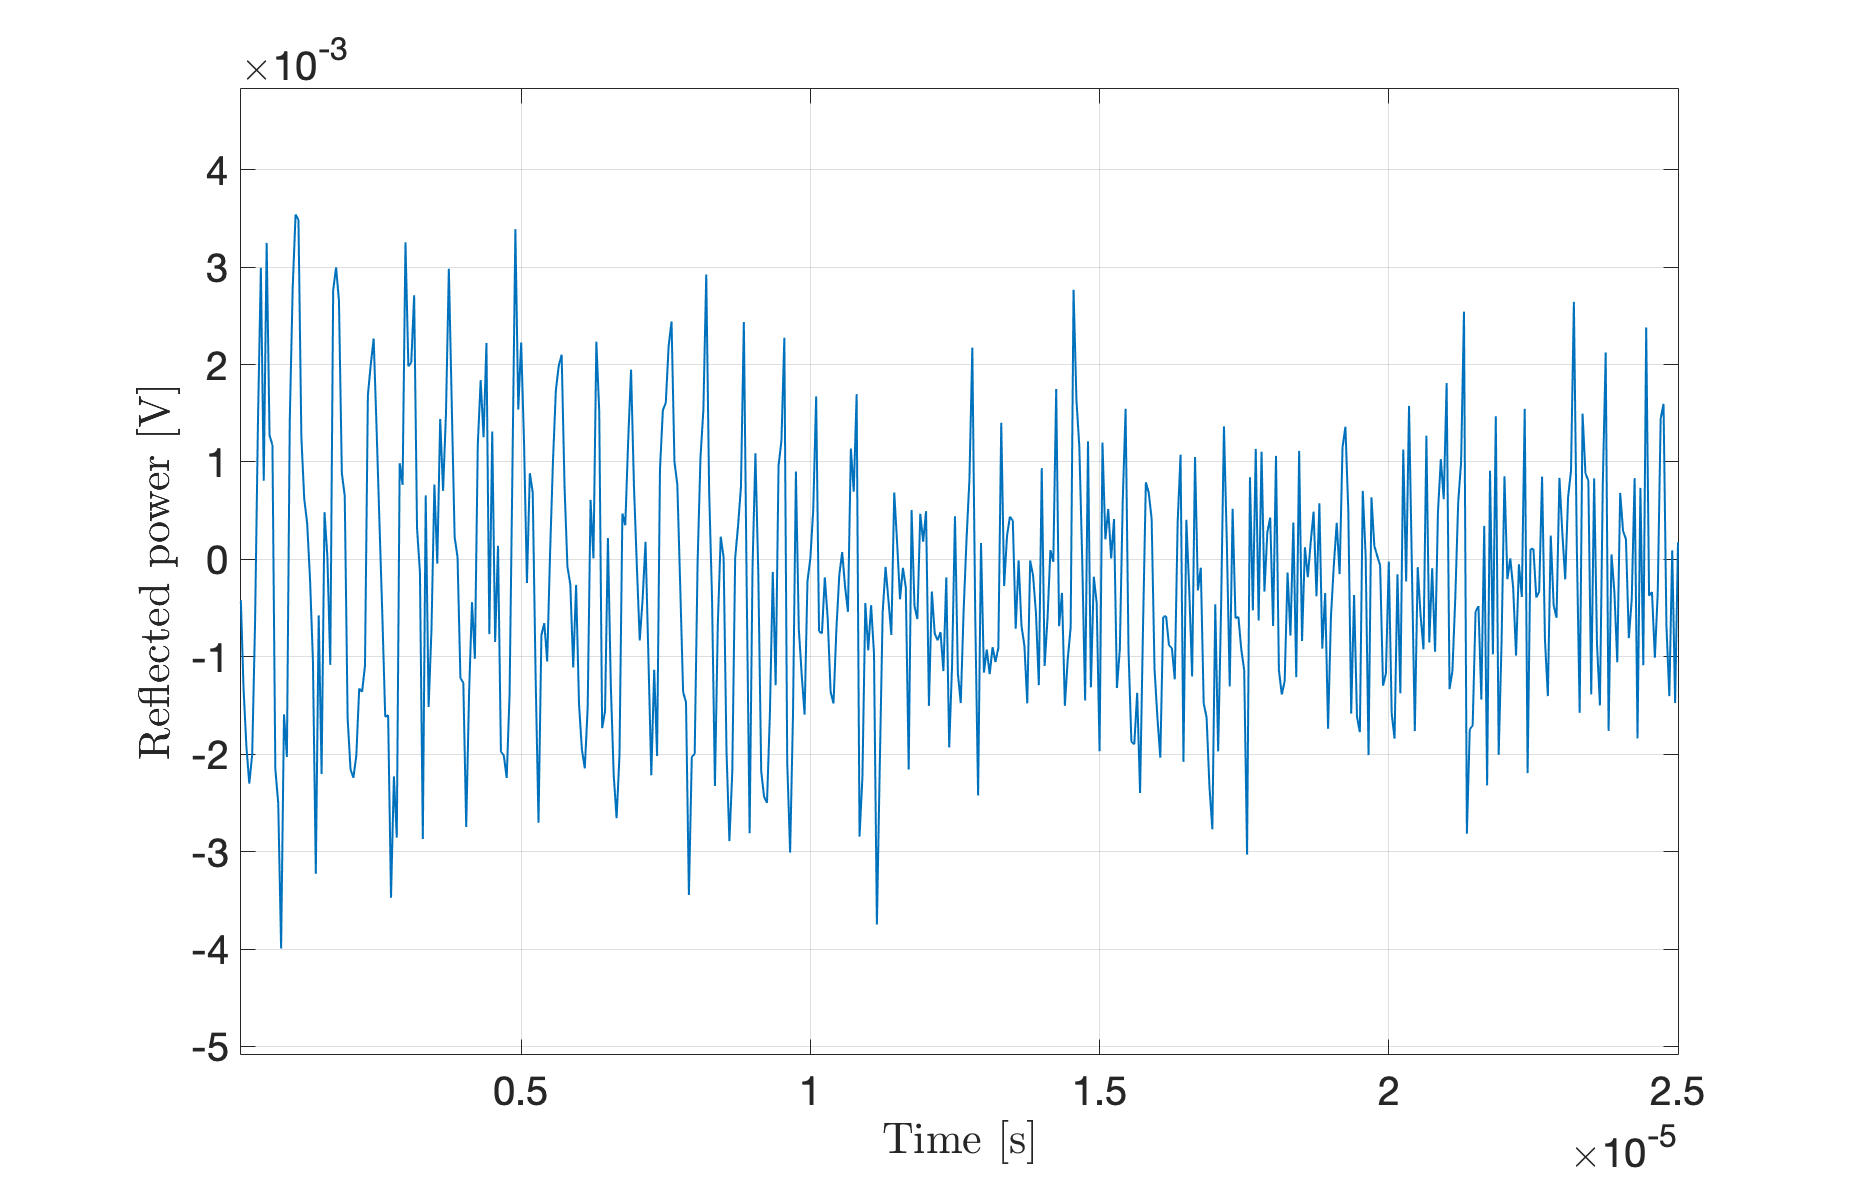
\includegraphics[width=.7\textwidth]{stab_mod/res.png}
	\caption{Residual reflected power [\si{\volt}] as a function of the time [\si{\second}] with $\tind{A}{PDH} = \SI{0.3}{\voltptp}$ and $\tind{\nu}{PDH} = \SI{1.56}{\mega\hertz}$ and with the reservoir stabilised at $\epsilon^* = \SI{300}{\au}$.}
	\label{stab_res}
\end{figure}

What is called the residual reflected power is the part of the fluctuations of the reflected power that is not due to the oscillations. It is defined as:

\begin{equation}
	\tind{V}{res}(t) = \tind{V}{ref}(t) - \tind{\mathcal{V}}{ref}(t)
\end{equation}

The residual power coming from the signals depicted on the figure \ref{stab_mod_signal} is shown in figure \ref{stab_res}. Once again, the previous formula can be used, provided that one uses $\tind{\sigma(\epsilon^*)}{res}$ (in \si{\volt}) instead of $\tind{\sigma(\epsilon^*)}{ref}$ to determine the phase noise based on the residual power $\tind{\sigma}{res}$ (in \si{\radian}):

\begin{equation}
	\tind{\sigma}{res} = \frac{\tind{\sigma(\epsilon^*)}{res}}{|\alpha_2|T_2}\pi
\end{equation}

% LONG TIME-SCALE PDH SIGNAL %

\subsubsection{Long time-scale Pound-Drever-Hall signal}

To be able to distinguish the modulation oscillations, the sampling frequency of the Digilock has to be at least twice the maximum \pdh modulation frequency, which is \SI{3.13}{\mega\hertz}, as required by the Shannon-Nyquist sampling theorem. To achieve higher sampling frequencies, the Digilock has to record data sets over shorter time-scales, as low as a few tens of microseconds, as can be seen on the time axis of the figure \ref{stab_res}, for example. The problem is that the duration of a \rcer experiment is in the order of the \si{\milli\second}. The long time-scale \pdh phase noise is simply a generalisation of the \pdh phase noise, but measured on a longer time-scale (\SI{5}{\milli\second}), to ensure the robustness of the stabilisation scheme over the long run. Let $\tind{\sigma(\epsilon^*)}{PDH,l}$ be the standard deviation of the \pdh error signal recorded over \SI{5}{\milli\second} (in \si{\au}). The long time-scale \pdh phase noise $\tind{\sigma}{PDH,l}$ (in \si{\radian}) is computed in exactly the same way as the \pdh phase noise, except that $\tind{\sigma(\epsilon^*)}{PDH,l}$ is used instead of $\tind{\sigma(\epsilon^*)}{PDH}$:

\begin{equation}
	\tind{\sigma}{PDH,l} = \frac{\tind{\sigma(\epsilon^*)}{PDH,l}}{|\alpha|T}\pi
\end{equation}

%%% RESULTS %%%

\subsection{Results}

The results of the measurements can be found in the tables of the appendix \ref{app-exp}. For each \pdh configuration and for each \pdh stabilisation position $\epsilon^*$, five data sets were measured in order to obtain results that are statistically more significant. In the tables, $\phi$, $\tind{\sigma}{PDH}$, $\tind{\sigma}{PDH,l}$, $\tind{\sigma}{ref}$, $\Delta \varphi$ and $\tind{\sigma}{res}$ are averages taken over the data sets, and $\mathcal{S}(\dots)$ are their respective standard deviations. The dimension of the different values is in \si{\milli\radian} unless specified otherwise.\\

 At the bottom of the tables, there is an additional row. It corresponds to the values obtained at a position indicated by $\epsilon^*$, but with a value of $k_I$ decreased to only \SI{500}{\volt\per\second}. This is done in anticipation of actual \rcer experiments for which this parameter needs to be smaller. During a run of the \rcer, the input power of the reservoir is modulated in intensity, therefore a change of the reflected power can be due to a variation of the input power, and not necessarily to a phase fluctuation. Decreasing the integral coefficient of the \gls{pid} makes it less likely to overreact to an intensity modulation. For each configuration, the stabilisation performance are only computed at one position, because this is done only to have a first idea of how a smaller $k_I$ impacts the reservoir.\\

For some $\epsilon^*$, there is an additional value called the \textit{challenger}, which is a heuristic used to determine the best stabilisation configuration and position. It is defined as the product:

\begin{equation}
	\text{Challenger} = \tind{\sigma}{PDH} \cdot \Delta \varphi
\end{equation}

Recalling that both $\tind{\sigma}{PDH}$ and $\Delta \varphi$ should be as small as possible, the best configuration is the one minimising the challenger. Note that there might exist more sophisticated heuristics leading to better results, but the challenger was used as a first approach thanks to its simplicity. The challenger was only computed for stabilisation positions for which the confidence in the measurements is the highest, and that are supposed to be usable in a practical \rc experiment. This condition excludes the positions:

\begin{itemize}
	\item For which a given value of $\epsilon^*$ can correspond to different phases.
	\item At which the slope of the transfer function is close to zero, which means that one is close to a minimum. This implies that linearising the transfer function at this point is not very relevant because this approximation rapidly becomes invalid, and that the phase noises deduced from this operation can be inaccurate.
	\item Where $\tind{\sigma}{PDH}$,  $\tind{\sigma}{PDH,l}$ and $\tind{\sigma}{res}$ are not included in an interval \SI{10}{\milli\radian} wide, all at the same time. When they are included, it increases the confidence in the measurements because it suggests that similar phase noises can be obtained in three different ways.
\end{itemize}

The five configurations and positions most likely to meet the criteria are presented in table \ref{ranking}. A striking feature emerging from these results is the fact the \pdh modulation frequency is the same for all the candidates. Therefore, when setting up a \rcer experiment, one should pay attention to use a \pdh modulation frequency of \SI{781}{\kilo\hertz}.

\begin{table}[h]
	\centering
	\begin{tabular}{|c|c|c|c|c|c|}
		\hline
		Rank & $\tind{A}{PDH}$ [\si{\voltptp}] & $\tind{\nu}{PDH}$ [\si{\kilo\hertz}] & $\epsilon^*$ [\si{\au}] & $\phi$ [\si{\radian}] & Challenger [\si{\milli\radian\squared}]\\
		\hline
		\hline
		\#1 & 0.4 & 781 & 400 & 1.3 & 1166\\
		\#2 & 0.2 & 781 & -300 & -1.43 & 1308\\
		\#3 & 0.4 & 781 & 700 & 1.45 & 1349\\
		\#4 & 0.3 & 781 & 500 & 1.31 & 1449\\
		\#5 & 0.4 & 781 & 600 & 1.39 & 1506\\
		\hline
	\end{tabular}
	\caption{Top-5 ranking of the positions and configurations}
	\label{ranking}
\end{table}

One important remark concerns the phase modulation amplitudes. In theory, for a given configuration, they should be constant, since $\tind{A}{PDH}$ is not changed. When looking at the data in appendix \ref{app-exp}, one notices that it is not the case, even when restricting the list of results to those with a challenger value (because one has more confidence on the quality of their measure). At this point, there is no satisfying explanation on why the modulation amplitude experiences position-dependent fluctuations. This incoherence can come from two main sources: the raw data measurement and the software post-processing. Regarding the former, most of the time during the measurements an external oscilloscope was plotting the different signals, and their shape agreed with the signals of the Digilock. This does not mean that an error on the measurements is impossible, but this increases the confidence that can be placed in them. Regarding the software used to analyse the results, there are two main components: the least square fitting of the sine function, and the slope estimator. The first is a function used as a black box leading to satisfying results, with a \SI{95}{\percent} confidence interval on the oscillation amplitude $\mathcal{A}$ very narrow (less than a percent relative to $\mathcal{A}$). This suggests that the failing component of the code is the estimation of the slope of the transfer function, even though the algorithm was always supervised while running, and did not seem to return aberrant results. One thing is certain, in the future, this phase modulation issue should be further investigated. This would benefit the whole experiment by making the characterisation results more solid.





